\documentclass[journal]{IEEEtran}

% Packages
\usepackage{amsmath,amsfonts,amsthm}
\usepackage{algorithmic}
\usepackage[caption=false,font=normalsize,labelfont=sf,textfont=sf]{subfig}
\usepackage{enumitem}
\usepackage{hyperref}
\usepackage{xcolor}
\usepackage{cite}
\usepackage{array}
\usepackage{graphicx}
\hyphenation{op-tical net-works semi-conduc-tor IEEE-Xplore}
\graphicspath{ {./img/} }
\newcommand{\BibTeX}{\textrm{B \kern-.05em \textsc{i \kern-.025em b} \kern-.08em
T \kern-.1667em \lower.7ex \hbox{E} \kern-.125emX}}
\usepackage{balance}

% Document
\begin{document}
    \title{Lessons Learned While Comparing Two Entity Resolution Models}
    \author{Andrei Olar}

    \maketitle

    \theoremstyle{definition}
    \newtheorem{defn}{Definition}[section]
    
    \maketitle
    \begin{abstract}
        \textcolor{green}{tb spus in 2 cuvinte ce inseamna ER}
        Despite well-established theoretical frameworks for entity resolution,
        there is a noticeable gap in its optimal application in practice.
        This framework 
        \textcolor{green}{care framework? prop precedenta zice de framework-uri in general...}
        plays a pivotal role in shaping the functionality of
        various metrics used to evaluate entity resolution algorithms.
        As a result, the interpretation derived from these metrics guides the
        determination of optimal input parameters for the algorithm under
        evaluation.
        This indicates that the practical projection of theoretical models in
        entity resolution often deviates from their optimal utilization, leading
        to varied outcomes and understandings of the problem.
        \textcolor{green}{tb mentionata si propunerea cu care vine acest paper; ce aduce el nou si care sunt concluziile studiului / investigatiei efectuate}
    \end{abstract}

    \begin{IEEEkeywords}
        Entity Resolution, Fellegi-Sunter, Algebraic Model, Metrics, Evaluation
    \end{IEEEkeywords}

    \section{Introduction}\label{sec:introduction}
    Entity resolution is the task of determining whether two information refer
    to the same real-world item or not.
    More restrictive definitions place entity resolution as the task of
    identifying and linking representations of data from two or more
    sources~\cite{Qia17}.
    However, we share the opinion that identifying and linking data constitutes
    a more specialized process~\cite{Tal11}.
    We also leave aside any classification 
    \textcolor{green}{of ???} 
    based on number of sources.
    The task of gathering information about a generic pound of potatoes across
    various marketplaces is still an entity resolution task, in our view.
    Whether the information about marketplaces and the potatoes that find
    themselves passing through there is available in one or more places strikes
    us as non-consequential, too.
    
    Because of its fundamental nature, the entity resolution problem goes by
    many names such as: record linkage, data de-duplication, merge-purge,
    named entity recognition and disambiguation, entity alignment or entity
    matching~\cite{Tal11,fever2009,alhelbawy2014}.
    Entity resolution also has many practical applications ranging from linking
    medical records to diagnosing diseases or ailments, to translation, to doing
    background checks for financial crime or to identifying plagiarism.
    Combining information from different media (sound, images, motion, smell,
    etc.) can also be regarded as a form of entity resolution when the purpose
    is to gather more information about the same real-world object.
    When there is such a wide array of past, present and future applications,
    evaluating entity resolution quality seems important.
    
    \textcolor{green}{aici e nevoie de:\\
    1. introducerea, pe scurt, a metodelor de evaluare din literatura, care sunt limitarile sau minusurile lor a.i. sa poti formula 1-2 research questions sau ipoteze pe care sa le valideze abordarea descrisa in articolul curent. Adica tb sa ai o motivatie pt toata munca efectuata;\\
    2. evidentierea contributiilor pe care le aduce lucrarea atat relativ la alte lucrari din literatura care analizeaza metrici si metode de evaluare (deci cu ce e diferita de ceea ce exista pana acum in literatura), cat si din punct de vedere al plusului efectiv de valoare adus de analiza efectuata}

    We begin by exploring a few preliminaries focused on entity resolution
    itself and then describe the problem we are analyzing.
    After briefly summarizing the work that relates to our paper, we introduce
    terminology and a mental model that we use throughout the rest of the paper.
    Following that we briefly introduce the theoretical models for entity
    resolution that we chose for our analysis.
    The experimental setup is next on our list as we present our findings using
    an algorithm of choice over three well known data sets as well as over one
    generated data set.
    Next, we discuss the results we see pointing out invariant conditions that
    do not seem to be related to the choice of data set.

    \section{Preliminaries}\label{sec:preliminaries}

    In scientific literature, entity resolution has been attributed numerous
    characteristics\cite{Tal11,Pap19}.
    In the current context, the following stand out:

    \begin{itemize}
        \item\textit{A concern for a real-world entity}, for if the task were
        not about a something from our world, there couldn't be any resolution;
        \item\textit{No implication as to the used method}, because if we
        stipulated a certain way to perform entity resolution, we might not be
        able to;
        \item\textit{The representation of information is computer friendly},
        because if it weren't, it might not be possible to study the task by
        means of computer science.
    \end{itemize}

    The first two statements suggest that entity resolution can be performed
    using any informational support.
    Simply imagine collecting notes about the same real-world object.
    Entity resolution's link with computer science exists only when posited.
    Dealing with information about real-world objects instead of dealing with
    the objects themselves directly~\cite{Tal11} doesn't transform entity
    resolution into a computer science problem.
    The self-imposed \textit{limitation} of dealing with information that is
    interpretable by a computer does.
    This entails that entity resolution tasks running on computers are not privy
    to the entities they are meant to resolve~\cite{Chen09}.

    Whenever we talk about measuring the performance of an entity resolution
    task, we must note that we are confined to the information that is available
    to the computer running the task.
    Our interests lie in bridging this gap between reality and approximation
    when it comes to the quality of entity resolution.

    It is said that beauty lies in the eye of the beholder.
    We are nearing a century since the date it has become apparent that the
    observer is key in our physical universe~\cite{schrodinger1926}.
    Perhaps we can use Schrodinger's insight as inspiration for bridging our own
    gaps in understanding entity resolution quality.
    For instance, we may 
    \textcolor{green}{say? notice?} 
    what are the perspectives available to us when we want
    to determine which information relates to the same real object.
    In other words, does it matter in practice how we model an entity resolution
    task theoretically?
    Is the observation of an entity resolution system made using a theoretical
    model the same or different than the one made using a different theoretical
    model and how?

    Historically, entity resolution measurements owe much to the field of
    information retrieval and statistics.
    Some of the measurements used to evaluate entity resolution quality seemed
    to faulter when put under scrutiny~\cite{Goga2015}.
    This 
    \textcolor{green}{gap or discrepancy or divergence} 
    leads to using better measures that describe the outcomes more wholly
    and more objectively.
    This 
    \textcolor{green}{I would add a noun for emphasising the incosistency of the evaluation setup available in literature} 
    indicates both that there is more than one lens to view entity
    resolution through and that the principles we should look for in such a lens
    should at least cover completeness and objectivity.
    
    \section{Question}\label{sec:contributions}

    Throughout the experience of working with entity resolution systems a few
    caveats become apparent.
    Firstly, adopting an entity resolution system is an arduous task at best.
    It is expensive in terms of consumed hardware resources, but also in terms
    of the manpower required to set up good data sets, data cleaning rules and
    entire data engineering processing pipelines.
    Because of this, finding optimal configuration parameters for entity
    resolution tasks quickly and cheaply is very desirable.
    Unfortunately, naively using `realistic' test datasets does not work often.
    Stellar outcomes on the test dataset often turn out much worse when the task
    is performed on production data.

    In this paper we would like to see what kind of perspectives over the task
    output we are granted by two theoretical models of entity resolution.
    Are there invariants we can glean on small scale data that we can transfer
    to larger, more chaotic data sets?
    More interestingly, are there invariants based in theory that we can
    transfer from one entity resolution algorithm to another?

    Breaking these larger questions down, we ask how much might a theoretical
    model influence the actual task's quality readout?
    That is, what is there to see past the numbers that we are shown when we
    measure the quality of an entity resolution task?
    Even more concretely, is the clustering performance of entity resolution
    correlated to the matching performance of entity resolution?
    Does the theoretical model we use determine how information should be
    represented at runtime?

    Zooming out again, we ask another question: is it possible to switch from
    one perspective to another?
    Entity resolution theoretical models encompass all entity resolution
    solutions: past, present and future.
    The abstract question above becomes whether we can interpret an entity
    resolution task's quality from a perspective that wasn't available at the
    time it was implemented or not?
    \textcolor{green}{aici nu e f clar la ce anume se refera aceste perspective. TBA}

    \section{Related Work}\label{sec:related}
    
    The topic addressed in this paper intersects with a significant body of
    existing research.
    Specifically, it aligns closely with three primary categories: presentations
    of entity resolution systems, theoretical model syntheses for entity
    resolution, and analyses of evaluation metrics in the field of entity
    resolution.

    Papers introducing entity resolution systems are relevant to this study due
    to their common objective of standardizing entity resolution tasks and their
    evaluation methods.
    The majority of the referenced systems in this context offer several generic
    metrics for assessing entity resolution performance.

    At the dawn of the 21st century, FEBRL~\cite{febrl2002} emerged as one of the
    first extensible systems to tackle measuring entity resolution performance.
    It was succeeded by FEVER~\cite{fever2009} and OYSTER~\cite{oyster2012}.
    These systems have all paved the way to generalizing our understanding about
    entity resolution and to ever more improvements in the quality of entity
    resolution tasks.
    Later on, systems like `Papers with Code'~\cite{papwithcode2019} brought in
    a social dimension to how we compare the qualitative performance of entity
    resolution tasks.
    The systems that came after, resemble frameworks more than they resemble
    applications~\cite{magellan2020,jedai2017}.
    Almost all systems are open-source and encourage social collaboration around
    entity resolution, too.
    
    Next, the syntheses on the theoretical models for entity
    resolution~\cite{fs1969,Ben2009Swoosh,Tal11} are invaluable resources.
    The models we present in this paper have been heavily documented before much
    better than we aspire to do here~\cite{Tal11,tal2013}.
    \textcolor{green}{It's nice to be humble, but here I would write another reason/motivation; the aim of the paper is to analize the evaluation component, not to re-describe the models; the models' description is given, in a uniform manner, just for improving the paper readability, fluency, comprehensibility}
    
    Taking a different tack on describing entity resolution in a generic,
    abstract way, we have studies that show a process perspective over entity
    resolution tasks~\cite{Pap19,Chen09}.
    These studies showcase the stages of the entity resolution process and the
    significance, challenges and benefits of each.
    With the help of such papers we find that matching and clustering are both
    sides of the same process as well as stages in it.

    Lastly, we use the information provided by syntheses~\cite{hitesh2012} on
    entity resolution quality metrics to find the metrics that associate well
    with a given theoretical perspective.
    For example, clustering or distance metrics do not describe well a
    probabilistic system.

    \section{Terminology}\label{sec:terminology}

    Throughout this paper the term ``entity'' is reserved for real-world items.
    We need new terms for the computer-friendly representations of entities.
    We start by saying that entity resolution operates on data sources.

    \begin{defn}
        A \textit{data source} represents a sequence of decoded messages
        that originate somewhere and can be processed by a computer program that
        reads them over a communication channel\footnote{The terms `decoded', `message' and `communication channel' refer to concepts
        defined in information theory~\cite{ash2012it}.}.
    \end{defn}

    
    
    An entity resolution task needs at least one data source to operate on.
    When the relevant information is split across multiple data sources, these
    can be merged into a single source.
    In the same way, a single data source can be split into multiple data
    sources.
    Data sources may be bounded (files or databases) or unbounded (streams).
    For the purposes of this paper, these attributes of data sources as well as
    their number are inconsequential.
    
    In the context of the definition of a data source, entity resolution is the
    computer program processing the data source.
    \textcolor{green}{Is ER a program? I recomend to consider it as a pb in the entire paper} 
    What sets entity resolution tasks apart from other computer programs are the
    notions they use to process information from the data source.

    \begin{defn}
        An \textit{attribute} is information about an entity that has a certain
        meaning in a context given by a frame of reference and certain rules of
        interpretation.
    \end{defn}

    Attributes by themselves are not enough to describe an entity.
    For example, `red' fully describes an entity only if we are looking for
    colors.
    If we are looking for fruit, `red' is only one of several attributes that
    help describe fruit.
    We might be interested whether the fruit is `sour' or `sweet' as well as
    whether it is `small', `medium' or `large'.

    \begin{defn}
        An \textit{entity reference} is a collection of attributes that refer
        to a real-world entity which can be formed by following an organizing
        principle (or order) of the data source where the attributes are all
        located.
    \end{defn}

    The organizing principle of a data source is simply an order that
    facilitates processing information in that data source.
    A CSV file has the organizing principle that attributes are separated by
    commas.
    Relational databases organize data in tables, columns and rows.
    Other storage organizes data in structured, semistructured or even
    unstructured ways (such as text).
    As an example of unstructured organization, named entity disambiguation uses
    the same organizing principle as named entity recognition built around
    mentions.
    When an entity resolution task processes a data source, it loads
    \textit{references}\cite{Ben2009Swoosh} to entities by taking advantage of
    the way that data source is organized.

    We shouldn't confuse the organizing principle of a data source with its
    structure, though.
    A table record in a database might store multiple attributes of the same
    entity in the same column.
    The entity reference will be constructed by extracting all attributes, not
    by dumbly considering each column to be an attribute.
    Entity reference extraction is also selective by nature.
    For entity resolution tasks that value geolocation above other things, the
    extracted references might skip over data that is not about geography.
    Similarly, in tasks that identify people, entity references will be
    comprised from attributes that are useful in identifying a person or a
    company.
    All this speaks to how the organizing principle of a data source is
    extrinsic to the data source and linked to the entity resolution's purpose.

    A final note on entity references is that attributes that each reference is
    bound to a data source.
    The definition above states this by mandating that all attributes comprising
    an entity reference are read from the same data source.

    So far we have dealt with structure, now it is time to deal with meaning and
    purpose.    
    Let's suppose that we are gathering information about colors.
    A data source represents colors as `red', `green' or `blue'.
    Another one represents them as \texttt{0xCC0000}, \texttt{00CC00} or
    \texttt{0x0000CC}.
    The organizing principle instructs the entity resolution task to construct
    entity references with a single attribute.
    It does not provide any semantic interpretation rules for the data.
    
    \begin{defn}
        A \textit{trait} is a semantic rule that guides the entity resolution
        task in recognizing the organizing principle of each information source
        that it uses as input.
    \end{defn}

    Each entity resolution task is defined by specific objectives it aims to
    achieve.
    For every distinct task, there are key rules that guide the interpretation
    of the available data, emphasizing certain aspects over others.
    In our example, entity resolution focuses exclusively on identifying colors
    in different data sources.
    To achieve this goal, the traits of the entity resolution task instance
    might be specified, trained or inferred from a knowledge base to recognize
    various representations of colours.
    While we might think of traits as being a part of a generic data extraction
    process such as scraping, traits in the sense described here are actually
    integral to the entity resolution process itself.
    
    The notion that is the most similar to that of a trait is the pattern
    recognition notion of a `feature':
    \textit{an individual measurable property or characteristic of a
    phenomenon}\cite{bishop2006pattern}.
    The mechanics of how traits and features function is near identical.
    The difference between a trait as defined here and a feature is a matter of
    perspective.
    Features are part of constructing a broader, objective perspective on
    information.
    Traits as they are defined here are concerned with the contextual meaning.
    
    Pragmatically, traits can be viewed as algorithms that extract information
    according to the subjective goal of the entity resolution task.
    In their simplest form, traits might be configuration parameters for an
    entity resolution system.
    But they can also be algorithms that are part of the a system's code.

    For example, a trait called `profitable' that is supposed to specify whether
    a company earns more than it spends is different from the typical physical
    representation of profit and loss as two separate decimal values present
    in information organized in some way or another.
    The way we would handle this discrepancy while extracting entity references
    is by having an algorithm that outputs a truth value when gains exceed
    spending.

    Another example of a trait, is a configuration value that specifies the
    attributes that should be used when comparing two entity references.
    This trait might optimize certain attributes of the entity references for
    comparison.
    
    To avoid confusing traits and attributes, it is easy to think about traits
    as not being a part of the data source, but rather as a part of the entity
    resolution task implementation.
    Entity resolution tasks extract attributes that they assign to entity
    references based on the traits specific to each task.

    Traits are a necessary abstraction if we want the same entity resolution
    task to be able to process more than one data representation.
    They are useful for constructing individual entity references.
    However, we have not defined any notion that links entity references to an
    entity.
    
    \begin{defn}
        The logical group of entity references that point to the same real-world
        entity according to the entity resolution task's parameters is known as
        the \textit{entity profile} of that real-world entity within the entity
        resolution task.
    \end{defn}

    It is important to understand that the entity profile and the real-world
    entity are not the same.
    Entity profiles are simply digital collections of entity references that are
    formed because of how an entity resolution task was programmed and
    configured.
    
    By using the terms \textit{information source}, \textit{attribute},
    \textit{trait}, \textit{entity reference} and \textit{entity profile} we can
    finally move on to define entity resolution formally.

    \section{Formalizing Entity Resolution}\label{sec:entity-resolution}

    In a broad sense, the entity resolution process is usually comprised of four
    different activities\cite{Pap19,Tal11}
    \textcolor{green}{I would use "steps" (instead of activities) in order to higlight their order - it is a process that involves all these 4 components}
    :
    \begin{itemize}
        \item \textit{entity reference extraction} --- the first phase of entity
        resolution deals with extracting entity references from multiple
        sources, as detailed  
        \textcolor{green}{in section \ref{sec:terminology}} 
        of this paper;
        \item \textit{blocking} and \textit{filtering} --- at this stage, the
        entity resolution task groups in the same `block' entities that share
        similar traits and then within each block all entities that cannot
        possibly match are filtered \textit{out}; the intent here is to allow
        entity resolution tasks to work with large amounts of data~\cite{Pap19};
        \item \textit{matching} --- one of the defining activities of the entity
        resolution process, it consists of comparing entity references to one
        another;
        \item \textit{clustering} --- the other defining entity resolution
        activity which collects matching references in entity profiles.
    \end{itemize}

    In this paper, we concern ourselves with the last two stages of the entity
    resolution process.
    \textcolor{green}{this decision must be motivated (a simple argument could be enough) - e.g. the focus is actually on the final evaluation}
    From now on, when we use the term \textit{entity resolution} we only refer
    to matching and clustering steps.

    However, because extraction plays a big part in how data is structured
    within any entity resolution process, we start specifying the entity resolution problem by formalizing the data extraction using the notions from
    Section~\ref{sec:terminology}.
    
    Given:
    \begin{itemize}
        \item $n \in N^*$ pairs ($S_i$, $n_i$), $1 \leq i \leq n$, $n_i \in N$, 
        where $S_i$ is a data source and $n_i$ is the number of messages in
        $S_i$,
        \item $m_i \in N^*$ traits $t_{ij}$, $1 \leq j \leq m_i$ for each
        information source $S_i$ so that
        \item each trait $t_{ij}$ can generate at most $a_{ij} \in N^*$
        attributes,
    \end{itemize}
    an entity resolution task $ER$ applies each trait $t_{ij}$ onto the source
    $S_i$, $1 \leq i \leq n$, $1 \leq j \leq m_i$, in order to extract
    $r_{{S_i}k}$ entity references where
    $0 \leq k \leq n_i \cdot \sum^{m_i}_{j=1}a_{ij}$.
    
    Next, we denote with $A$ the domain of all possible attributes that can be
    used by $ER$.

    In this context, let $r_{{S_i}{k_j}}$ denote the $k_j$th, $1 \leq j \leq k$
    entity reference extracted from the source $S_i$.
    Then $r_{{S_i}{k_j}}$ is a tuple
    \[
        (a_r, r \in N^*, a_r \in A), r_{{S_i}{k_j}} \in A^r
    \]
    where $r$ varies for each $k_j$.

    Defining traits and the organizing principle as external to the data source
    is what allows us to formalize entity references so simply.
    A trait is then a function that helps construct entity references.
    The definition of traits materializes only upon extracting entity references
    $r_{{S_i}{k_j}}$ with $ER$.
    The domain of this function is the domain of all attributes in the source
    $S_i$.
    We denote this domain with $A_{{S_i}{k_j}}$.
    
    A trait can be declared as a function:

    \[
        t: S_i \rightarrow A_{{S_i}{k_j}}^x\textrm{, where }x \in N^*
    \]
    and $x$ varies with $k_j$.

    During the extraction process, \textit{ER}'s traits lead to the construction
    of the domain of entity references:

    \[
        Ref = \bigcup_{i \in N^*,1 \leq j \leq k} r_{{S_i}{k_j}}
        \textrm{, with } r \textrm{, }S \textrm{ and } k \textrm{ specified above.}
    \]

    The $Ref$ domain is constructed through entity reference extraction.
    After the entities have been extracted, we are no longer concerned with the
    input information sources.
    Every type of entity resolution task can be made to work on such an input
    domain~\cite{Pap19}.
    De-duplication tasks that use a single data source work out of the box.
    Record linking tasks that use two or more data sources can embed an
    attribute that identifies the data source of each entity reference.
    Regardless of the optics, the input domain contains only entity references.
    The relevance of the original data source of an entity reference rests with
    the entity resolution task and its matching and clustering algorithms.

    The output of entity resolution is always a collection of entity profiles.
    While the data representation of an entity profile is definable only per
    theoretical model, we can define the output domain of entity resolution

    \[
        Res=\{P_x \mid x \in \mathbb{N^*}, P_x \in P\}
    \]

    \noindent
    as the domain of collections of entity profiles.

    This specification, finally, allows us to formalize entity resolution itself as a function:

    \[
        e(r_1, r_2, \ldots, r_n): Ref^n \rightarrow Res\text{, where }n\in\mathbb{N^*}
    \]
    
    \noindent
    which takes in a sequence of entity references and outputs a sequence of
    entity profiles.

    Note that $Res$ is always going to be a collection containing unique entity
    profiles in any theoretical model of entity resolution because of the nature
    of the entity resolution problem.
    Entity resolution disambiguates information, making it impossible for
    identical items to be a part of its output.
    This should not be taken to mean that the output of entity resolution tasks
    will always be a set of profiles.

    If $Res$ is the domain of all collections of entity profiles, one of
    these sequences 
    \textcolor{green}{which ones?} 
    must be the ideal one.
    The ideal collection of entity profiles contains the approximation which is
    closest to our understanding of the real world items represented by the
    entity profiles.

    \begin{defn}
        We define the \textit{ground truth} \textbf{G} over the entity reference
        domain \textit{Ref} as the entity resolution result comprised of entity
        profiles:
        \[
            \{P_g \mid g \in \mathbb{N^*}\}\textrm{, such that:}
        \]
        \begin{itemize}
            \item each $P_g$ describes an entity completely using the available
            entity references from $Ref$, and
            \item there are no entity references in \textit{Ref} which are not a
            part of a $P_g \in G$.
        \end{itemize}
    \end{defn}

    In other words the ground truth is the ideal entity resolution result for 
    the given input data, in a context, from a perspective.
    Knowing this, we can formalize entity resolution quality generically with
    respect to the ground truth.
    
    \begin{defn}
    Given an entity resolution \textit{e} and the ground truth \textit{G} for
    the entity reference domain $Ref$, a \textit{quality metric} is an
    idempotent function:
    \[
        q(G, Res_e): Res^2 \rightarrow \mathbb{R}\textrm{, where
        }Res_e\textrm{ is the result of }e
    \]
    scores how similar the result of \textit{e} is to \textit{G}.
    \end{defn}
    \textcolor{green}{oare nu e confuz sa se noteze cu e si o functie (2 ecuatii mai devreme) si si ca indice?? Imi scapa mie ceva oare?}

    In practice, we should strive to implement quality metric as \textit{pure}
    functions, guarding their execution from any side-effects specific to
    running a program on a computer.

    As stated before, the shape and structure of the items in $Res$, including
    $G$, depends on the mathematical model underpining a specific entity
    resolution task implementation.
    Because the input domain of the quality metrics changes according to the
    used mathematical model, the set of quality metrics available for describing
    the performance of a certain entity resolution task $Q = \{q_y \mid y \in
    \mathbb{N}\}$ is dependent on the mathematical model used for implementing
    that task.

    One possible answer to the question of whether it is possible to evaluate
    an entity resolution using a theoretical model which wasn't available at the
    time when the entity resolution was designed has to do with the
    applicability of quality metrics.

    A simple logical inference tells us that if two theoretical models represent
    entity profiles in the same way, they also share quality metrics.
    Essentially, if the entity resolution $e_1$ can be evaluated using a set of
    quality metrics $Q_1$ and $e_2$ can be evaluated using a set of quality
    metrics $Q_2$ such that $Q_1 \cap Q_2 \neq \emptyset$, we have a set of
    quality metrics $Q_\cap = Q_1 \cap Q_2$ that allows us to compare $e_1$ and
    $e_2$ based on $Q_\cap$.
    
    \section[mm]{Mathematical Models for Entity Resolution}\label{sec:mm}

    The representation of entity resolution results depends upon the theoretical
    model we use.
    There are multiple theoretical models available for entity resolution and
    they range from ones based on complex networks and graph theory\cite{Li2020}
    to ones based on probabilities\cite{fs1969} or
    algebra\cite{Tal11,Ben2009Swoosh}.

    John R. Talburt provides an overview of these models in his book ``Entity
    Resolution and Information Quality''\cite{Tal11}.
    This paper aims to take a deeper look at how two of the models described
    therein might be connected.

    \textcolor{green}{e nevoie sa argumentezi de ce te-ai oprit doar asupra acestor 2 modele din multimea celor existente!}

    \subsection[fsm]{Fellegi-Sunter Model}\label{subsec:fsm}

    In the late 1960s Ivan Fellegi and Alan Sunter wrote the seminal
    paper\cite{fs1969} for what was called record linkage and would later become
    known as entity resolution.
    To this day, the probabilistic model for entity resolution is this problem's
    most popular formalization.
    In this mathematical model, entity resolution is a function that aids in 
    probabilistic decision making.
    
    \subsubsection[fsm-desc]{Description}\label{subsubsec:fsm-desc}

    The original Fellegi-Sunter (F-S) model defines record linkage as an operation over two input
    sets, $A$ and $B$.
    The result of the operation is a set containing pairs of items
    $X = \{(a, b), a \in A, b \in B\}$ or $X = A \times B$.
    
    The model then deconstructs $X$ to two disjoint subsets $X = M \cup U$:
    \begin{itemize}
        \item $M$ for pairs that contain matching items, and
        \item $U$ for pairs that contain non-matching items,
    \end{itemize}
    or more formally:
    \begin{align}
        M &= \{(a, b) | a == b, a \in A, b \in B\}~\textrm{and}\nonumber \\
        U &= \{(a, b) | a \neq b, a \in A, b \in B\}\nonumber
    \end{align}

    The model proposes that if $a \in A$ and $b \in B$ are two vectors, their
    comparison will also be a vector denoted $\gamma \in \varGamma$, where
    $\varGamma$ denotes the set of all possible values of $\gamma$.
    The comparison between $a$ and $b$ is performed between each corresponding
    element in each of the two vectors.
    The elements of $\gamma$ vary according to the type of comparison that is
    performed\cite{winkler1990}.

    In this context, a match decision function can make one of three decisions
    regarding a pair from $X$ according to the F-S model:
    
    \begin{itemize}
        \item consider it a \textit{link ($A_1$)} between the items;
        \item consider it a \textit{non-link ($A_3$)} between the items, and
        \item leave things undecided, thus marking it as a \textit{possible link
              ($A_2$)}.
    \end{itemize}
    
    Then a linkage rule is a function $L:\varGamma \rightarrow D$,
    $D=\{d(\gamma)\}$, where
    
    \begin{align}
        d(\gamma) = &\{P(A_1|\gamma),P(A_2|\gamma),P(A_3|\gamma)\}\textrm{, so
        that:}\nonumber\\
        &\sum_{i=1}^{3}P(A_i|\gamma) = 1\nonumber, \gamma \in \varGamma\nonumber
    \end{align}

    In other words, given a $\gamma \in \varGamma$, we have the linkage rule
    \[
        L(\gamma) = \{P(A_1|\gamma), P(A_2|\gamma), P(A_3|\gamma)\}
    \]
    so that the probabilities sum up to $1$.

    When using this model the purpose of entity resolution is to find the
    optimal linkage rule.
    The F-S theorem defines it as the linkage rule that minimizes
    $P(A_2|\gamma)$.
    In other words, the optimal linkage rule according to the F-S model is the
    linkage rule without uncertainties.
    This inclination of this model towards optimization makes it well suited for
    both rule-based\cite{oyster2012} and machine learning\cite{deepm2020}
    implementations.
    
    In the probabilistic model, two conditional probabilities are interesting:

    \begin{align}
        m(\gamma)&=P(\gamma(a, b) | (a, b) \in M)~\textrm{and}\nonumber\\
        u(\gamma)&=P(\gamma(a, b) | (a, b) \in U)\textrm{.}\nonumber
    \end{align}

    \noindent
    $m(\gamma)$ is the probability of a $\gamma$ comparison vector given an
    $(a, b)$ \textit{link}.
    $u(\gamma)$ is the probability of a $\gamma$ comparison vector given an
    $(a, b)$ \textit{non-link}.
    For brevity, we have not used the complete notation pertaining to records
    from the original paper.

    The two probabilities outlined above are important because they help us
    express the probabilities of the Type I and Type II statistical errors
    associated with the decision function that sits at the core of the linkage
    rule definition above.
    The probabilities of the two types of error are expressed as:

    \begin{align}
        \mu&=\sum_{\gamma \in \varGamma}u(\gamma)P(A_1|\gamma)\textrm{,~and}\nonumber\\
        \lambda&=\sum_{\gamma \in \varGamma}m(\gamma)P(A_3|\gamma)\nonumber
    \end{align}

    where:

    \begin{itemize}
        \item $\mu$ represents the Type I error of items that were erroneusly
        linked (i.e pairs in $M$ that do not belong in $M$), and
        \item $\lambda$ represents the Type II error of items that were
        erroneously \textit{not} linked (i.e~pairs in $U$ that do not belong in
        $U$).
    \end{itemize}


    \textcolor{green}{some remarks:\\ 
    1. While Fellegi and Sunter show that the classification rule is optimal in terms of statistical power, the result is based on several assumptions that do not hold in practice - check this work \href{https://www.jstor.org/stable/23024863?seq=1}{link}\\
    2. there are some generic versions of FS model - e.g. \href{https://www.jstor.org/stable/pdf/24246450.pdf}{link}, \href{https://projecteuclid.org/journals/annals-of-applied-statistics/volume-8/issue-4/Detecting-duplicates-in-a-homicide-registry-using-a-Bayesian-partitioning/10.1214/14-AOAS779.full}{link}\\
    }

    \subsubsection[fms-term]{Terminology Mapping}\label{subsubsec:fsm-term}

    To link the Fellegi-Sunter model to our own terminology, let's start by
    talking about $a \in A$ and $b \in B$.
    The F-S model calls $A$ and $B$ ``populations'' and $a$ and $b$,
    ``population elements''.
    A distinction is made between records, denoted with $\alpha(a)$ and
    $\beta(b)$, and population elements.
    Most of the original paper refers to records.

    Population elements correspond to entities and records correspond to entity
    references in our terminology.
    When it comes to $\alpha(a)$ and $\beta(b)$, we think of them as special
    cases of traits.
        
    The $A$ and $B$ populations equate to data sources.
    A ``population'' is a particular type of data source because it is defined
    as a set.
    The set is a specialization with respect to our definition of data sources.
    
    The Fellegi-Sunter model works under the assumption that there are two
    populations $A$ and $B$ and defines the linkage rule as a function that uses
    conditional probabilities that involve both populations.
    On the other hand, our $Ref$ domain is solitary.
    Using our terminology we would denote $A$ with $S_1$ and $B$ with $S_2$.
    We start constructing our $Ref$ domain by using traits to extract $n_1$
    entity references from $S_1$ and $n_2$ entity references from $S_2$.
    Then $Ref = \{r_{{S_i}{k_j}},~1 \leq k_j \leq n_i, i \in {1, 2} \}$.
    If, say there is 5 elements in $S_1$ and 10 elements in $S_2$ then $k_1$ goes
    from 1 to 5 and $k_2$ goes from 1 to 10.

    The result domain is expressed as $X = A \times B$ in this model.
    It is subsequently split into $M$ and $U$ the sets of matching and
    non-matching pairs in $X$, respectively.

    The $X$ in the original model is equivalent to $Res$ in our terminology.
    $Res$ can be defined as:
    \begin{align}
        Res = &\{(r_{{S_i}{k}}, r_{{S_j}{l}})\mid~1 \leq k \leq |S_i|,
        1 \leq l \leq |S_j|\}\textrm{, so that}\nonumber\\
        &i \neq j, i,j \in \{1, 2\}\textrm{,}\nonumber
    \end{align}
    where $|S_i|$ denotes the number of entity references extracted from the
    source $S_i$.

    Each entity profile is represented as a pair of entity references.
    For example, if $r_{11}=(1, 2, 3)$ and $r_{21}=(4, 5, 6)$ are two entity
    references that refer to the same real-world entity, this model would return
    an entity profile as the following pair: $((1, 2, 3), (4, 5, 6))$.

    $M$ becomes the set containing the entity profiles that refer to entities.
    $U$ becomes the set of entity profiles that don't refer entities.
    Consequently, this model proposes that the result of entity resolution is a
    set of distinct pairs of entity references.

    A natural question is whether, instead of a single set of pairs of tuples we
    should expect two sets of pairs of tuples that would correspond to the two
    subsets $M$ and $U$ from the original paper.
    $M$ will grow proportionally to the maximum number of entity references
    extracted from a single data source.
    On the other hand, the size of $U$ is proportional to the product of the
    sizes of the populations $A$ and $B$.
    For practical reasons concerning resource usage, we think constructing $M$
    and inferring $U$ based on $M$ is the best choice.

    With the above definition for $Res$ we observe that this model explain
    matching very well, but clusters entities only two at a time.
    Linking more than two entity references, and especially implementing
    transitive entity reference linking does not seem possible with this
    model\cite{Tal11}.
    By transitive linking we mean that if the entity reference $r_1$ matches
    $r_2$ and $r_2$ matches $r_3$, we could infer that $r_1$ matches $r_3$.
    While there is work that extends the model to compare more than two entity
    references\cite{Kon19} at once, transitivity is still an issue so we will
    not dive deeper into topics concerning matching multiple entity references.
    
    \subsubsection[fsm-metrics]{Specific Metrics}\label{subsubsec:fsm-metrics}

    Because we have a clear definition of the Type I and Type II errors, we can
    give a clear context for the notions of true and false positive and true and
    false negative.
    This allows us to use any of the familiar statistical metrics that rely on
    these concepts.
    
    In defining true/false positives/negatives we use the sets $M$ and $U$ as
    they are defined in the original paper describing the F-S model.
    Depending on where a pair (output by the entity resolution function) is
    expected to be found, we define:

    \begin{itemize}
        \item \textbf{true positives} as pairs predicted to be in $M$ that
        should be in $M$,
        \item \textbf{false positives}, or type I errors, as pairs predicted to
        be in $M$, but should be in $U$,
        \item \textbf{true negatives} as pairs predicted to be in $U$ that
        should be in $U$, and
        \item \textbf{false negatives}, or type II errors, as pairs predicted to
        be in $U$, but should be in $M$.
    \end{itemize}

    Quality metrics for this model compare a ground truth, consisting of ideal
    tuple pairs, with the entity resolution task's output.
    $M$ is the ground truth in this context.
    Due to the impracticality of using $U$, our focus will be on concepts
    related to $M$: true positives, false positives, and false negatives.
    
    Several metrics based on these concepts exist, though the effectiveness of
    some has been questioned\cite{Goga2015}.
    With this in mind we choose three quality metrics that are widely used with
    this model:

    \begin{align}
    Precision &= \frac{TP}{TP+FP}\nonumber \\
    Recall &= \frac{TP}{TP+FN}\nonumber \\
    F_1 &=2 \cdot \frac{Precision \cdot Recall}{Precision+Recall}\nonumber
    \end{align}

    \textit{Precision} (or the positive predictive value) is defined as the
    number of correct predictions that were made in relation to the total number
    of predictions that were made.

    \textit{Recall} (or sensitivity) is defined as the number of correct
    predictions that were made in relation to the total number of positive
    predictions that could have been made (which corresponds to the number of
    items in the ground truth).

    The \textit{$F_1$} score is the harmonic mean of the precision and the
    recall and it is used to capture the tradeoff between precision and
    recall\cite{hitesh2012}.

    \textcolor{green}{e bine ca pentru fiecare metrica sa fie precizat domeniul valorilor posibile si ce inseamna bine (predictii bune) si ce inseamna rau (predictii gresite)}

    \subsection[algebraic]{Algebraic Model}\label{subsec:algebraic}

    Initially proposed as a model to discern information quality in entity
    resolution over large datasets\cite{tal2007algebraic}, the algebraic model
    for entity resolution was later refined to describe entity resolution
    itself\cite{Tal11}.
    While the Fellegi-Sunter model described in Subsection~\ref{subsec:fsm} is a
    probabilistic model that partitions input in two data sources to compare,
    this model allows as many information sources as necessary.
    Another improvement is the support for transitive matching.
    
    \subsubsection[algdesc]{Description}\label{subsubsec:algdesc}

    The core tenet of this model is that entity resolution is an \textit{
    equivalence relation}, in the sense defined in set theory.
    
    \begin{defn} If $X$ is a set and $R$ is a rule that takes two elements from
    $X$, $x$ and $y$, and tells us whether $x$ is in relationship $y$ in the way
    denoted with $R$, then we call $R$ a \textit{binary relation} on
    $X$\cite{hoffman1971linear}.
    \end{defn}

    We can represent $R$ as a function $R:X \times X \rightarrow \{0,1\}$ where
    $R(x,y)=1$ if $x$ is in relation $R$ with $y$ and $R(x,y)=0$ otherwise.
    
    \begin{defn}If $R$ is a binary relation on the set $X$, it is convenient to
    write $xRy$ when $R(x, y) = 1$.
    A binary relation R is called:

    \begin{enumerate}
        \item reflexive, if $xRx, \forall x \in X$;
        \item symmetric, if $yRx \implies xRy$, $\forall x,y \in X$;
        \item transitive, if $xRz \land yRz \implies xRz$, $\forall x,y,z \in X$.
    \end{enumerate}

    An \textit{equivalence relation} on $X$ is a reflexive, symmetric, and
    transitive binary relation on $X$\cite{hoffman1971linear}.
    \end{defn}

    Note that equivalence relations seem to describe almost perfectly the
    matching step in entity resolution.
    Let's also observe that equivalence relations work on sets for now and move
    on.

    An equivalence relation over a set $X$ generates an equivalence class.

    \begin{defn}Suppose $R$ is an equivalence relation on the set $X$.
    If $x$ is an element of $X$, let $\bar{x}$ denote the set
    $\{y \in X | xRy\}$.
    $\bar{x}$ is called the \textit{equivalence class} of $x$ (for the
    equivalence relation $R$)\cite{hoffman1971linear}.
    \end{defn}

    Since $R$ is an equivalence relation, the equivalence classes for $R$ have the
    following properties\cite{hoffman1971linear}:
    \begin{enumerate}
        \item $xRx \in \bar{x} \implies \bar{x} \neq \emptyset$,
        \item $y\in\bar{x}\iff~x\in\bar{y}$,$~\forall x,y \in X$ because
        equivalence relations are symmetric,
        \item $\forall x,y \in X$, $\bar{x}$ is either identical with $\bar{y}$
        or they have no elements in common\cite{hoffman1971linear,Tal11}.
    \end{enumerate}
    
    The last fundamental notion from set theory that is needed to construct the
    algebraic model of entity resolution is the \textit{partition} of a set.

    \begin{defn}
        A \textit{partition} of a set $X$ is a collection of non-empty disjoint
        subsets of $X$ whose union is $X$\cite{halmos1960naive,Tal11}.
    \end{defn}

    Things come together starting with the simple observation that an element
    belonging to one of the sets from a partition over $X$ is in a relation with
    itself and other elements from the same set.
    We say that this relation is \textit{induced} by the partition.
    Conversely, from the point of view of the above relation, we say that it
    \textit{generated} the partition.

    When the partition in question is the set of equivalence classes over $X$,
    then the induced relation is an equivalence relation.
    Conversely, an equivalence relation $R$ in $X$ will generate a partition
    over $X$ comprised by the equivalence classes of $X$\cite{halmos1960naive,
    Tal11}.

    \begin{defn}
        The equivalence relationship over a set of entity references that exists
        when two references from that set refer to the same real-world entity is
        called \textit{entity resolution}.
    \end{defn}
    \textcolor{green}{daca aici ai dat definitia ER in stilul modelului algebric, ar fi bine sa incluzi si la modeulul F-S o definitie pt ER in termenii F-S}



    Let's denote this relation with $ER$ and state that if $xERy$ then x and y
    are \textit{linked}\cite{Tal11}.
    Taking our two earlier mental notes, we can now say that applying $ER$ to
    individual elements of a set is akin to the \textit{matching} step in the
    entity resolution process.
    With each application, we now know that $ER$ creates a partition over the
    initial set.
    This side-effect of equivalence relationships is the \textit{clustering}
    step or aspect of the entity resolution process.
    The equivalence classes from the partition generated by $ER$ are also known
    as \textit{clusters} in the context of entity resolution.
    \textcolor{green}{similar cu obs precedenta; ar fi bine ca si pt modelul F-S sa fie prezentata aceasta corespondenta dintre model si cei 4 pasi ai procesului ER}

    A last point of notice is that entity resolution tasks do not necessarily
    generate a unique outcome\cite{Tal11}.
    Depending on the order in which entity references are processed, runing the
    same entity resolution task might generate different partitions.
    The entity resolution tasks where the order in which entity references are
    processed is irrelevant are called \textit{sequence neutral}\cite{Tal11}.
    In this paper we are only interested in sequence neutral entity resolution
    tasks.
    \textcolor{green}{similar cu obs precedenta; ar fi bine ca si pt modelul F-S sa fie prezentata aceasta perspectiva legata de cardinalitatea iesirilor}

    \subsubsection[algrel]{Terminology Mapping}\label{subsubsec:algrel}

    In writing this paper, we used a lot of notions that are specific to the
    algebraic model.
    For example, attributes and entity references preserve their meaning.
    In fact, it can be safely assumed that all common terms preserve their
    meaning.
    
    This paper's terminology is divergent when it comes to our use of
    information sources and our attempts to generalize data structures and the
    entity resolution process itself past the limits of the algebraic model.
    For example, information sources contain an inordinate amount of duplicate
    data, incomplete data or noise.
    The algebraic model can't function under those circumstances.
    Therefore, whenever we refer to the input source for the algebraic model,
    we are referring to a set of entity references containing clean data.
    
    We also should note that the algebraic model does not concern itself with
    how entity references end up being part of the same set, just that they do.
    Therefore using different traits (in the sense of this paper) will lead to
    different outcomes.
    In fact, the only place where we feel traits might be important in relation
    to the algebraic model is with regard to the sequence neutrality of an
    entity resolution task.
    In our view, an entity resolution task's sequence neutrality can be tested
    by using separate sets of traits that change the order in which items are
    fed to the entity resolution task.

    The result of an entity resolution task is a partition over the input set of
    entity references.
    This defines the output domain of our entity resolution function as:

    \begin{align}
        Res &= \{C_1,~C_2,~C_3,~\ldots,~C_n\mid~C_i\in~P\}\textrm{, so that}\nonumber\\
        C_i&\neq\emptyset,\forall~1\leq~i\leq~n\textrm{,~and}\nonumber\\
        C_i\cap~C_j&\neq\emptyset,\forall~1\leq~i\neq~j\leq~n\textrm{,~and}\nonumber\\
        \bigcup_{i=1}^{n}C_i&=Res\nonumber
    \end{align}

    Another way to read the above definition is that ground truth and all other
    entity resolution results are partitions over $Ref$.
    The definition also implies that any entity reference in $Ref$ will be a
    part of only one cluster.
    Each equivalence class in an entity resolution result is a cluster of entity
    references.
    A cluster of entity references is an entity profile.

    \subsubsection[algeval]{Specific Metrics}\label{subsubsec:algeval}

    The quality metrics for entity resolution under the algebraic model have to
    do with computing the similarity of partitions.
    In our case, these metrics are applied to compare the partitions $G$ and
    $Res$.
    Many such metrics exist\cite{hitesh2012} and we chose to cover some of them
    which either by lineage or by their popularity have peaked our interest.

    The first among these is the Rand index introduced by William Rand in
    1971\cite{rand1971}.
    This index computes the similarity of partitions by comparing pairs of
    elements formed from the elements of the clusters of each partition.
    Supposing that:
    \begin{itemize}
        \item $a$ is the number of pairs that are shared between clusters of $G$
        and $Res$,
        \item $b$ is the number of pairs that are only in clusters in $G$, but
        not in clusters in $Res$,
        \item $c$ is the number of pairs that are only in clusters in $Res$, but
        not in clusters in $G$,
        \item $d$ is the total number of pairs that are not shared.
    \end{itemize}
    then the Rand index is defined by the quantity
    $\frac{a+d}{a+b+c+d}$\cite{adjrand2001}.

    The minimum value of the Rand index is 0, meaning nothing matches, while its
    maximum value is 1, indicating a perfect match.
    The obvious use of the Rand index is to rate the similarity of two
    partitions.
    Its less obvious use is to consider $1 - Rand Index$ the distance between
    two partitions.

    The expected value of the Rand index of two random partitions does not take
    a constant value (say zero)~\cite{adjrand2001}.
    That lead to the introduction of the adjusted Rand index which follows the
    same principles, 
    \textcolor{green}{adica 0 inseamna no match si 1 perfect match? sau la ce anume te referi prin "same principles"?}
    but uses a specific distribution for
    randomness~\cite{adjrand1985}.
    Without going into detail, we can provide a formula for the adjusted Rand
    index by using the quantities we defined for the Rand index~\cite{Tal11}.
    \[
        Adjusted~Rand~Index = \frac{
            a -\left(\frac{(a+b)\cdot(a+c)}{a+b+c+d}\right)
        }{
            \frac{(2\cdot a+b+c)}{2}-\left(\frac{(a+b)\cdot(a+c)}{a+b+c+d}\right)
        }
    \]
    \textcolor{green}{tb precizat domeniul de valori posibile si ce inseamna valoare buna si valoarea rea}

    The third quality metric we can use for comparing partition similarity is
    the Talburt-Wang index (TWI).
    The merit of this metric is that it closely follows the Rand index, but is
    much simpler to compute~\cite{Tal11}.
    \[
        TWI = \frac{\sqrt{|G|\cdot|Ref|}}{|G \cap Ref|},
    \]
    where if $X$ is a set, then $|X|$ represents the numer of elements in $X$. 
    The TWI uses the number of clusters that are found in both the ground
    truth and in the entity resolution task's output.
    It provides a good approximation of how many clusters are returned correctly
    by the entity resolution task.
    The Talburt-Wang index takes values between 0 and 1, with 1 indicating that
    the return value of the entity resolution task perfectly matches the ground
    truth.

    Other similarity metrics used to compare partitions are the pairwise and
    cluster precision and recall metrics.
    They were first introduced in 2010 as an alternative quality
    metrics to be used for evaluating entity resolution results\cite{Men10}. 
    \textcolor{green}{eu as include si referintele "radacina": https://www.jstor.org/stable/pdf/1756667.pdf, https://www.cs.utexas.edu/users/ml/papers/marlin-kdd-wkshp-03.pdf}

    Similarly to the Rand Index, pairwise metrics rely on extracting pairs of
    items to determine how similar two set partitions are.
    They differ from the Rand index because pairwise metrics operate at the
    partition level and not at the partition class level.
    
    Pairwise precision (denoted \textit{PP}) is defined as the ratio between the
    number of pairs in $Res$ that are also in $G$ and the number of pairs in
    $Res$.
    In other words pairwise precision tells us how many pairs the entity
    resolution task got right out of the pairs it returned.
    \[
        PP = \frac{|Pairs(Res) \cap Pairs(G)|}{|Pairs(Res)|}
    \]
    \textcolor{green}{tb precizat domeniul de valori posibile si ce inseamna valoare buna si valoarea rea}

    Pairwise recall (denoted \textit{PR}) is defined as the ratio between the
    number of pairs in $Res$ that are also in $G$ and the number of pairs in $G$.
    In other words, pairwise recall tells us how many pairs the entity
    resolution task got right from the ideal answer.
    \[
        PR = \frac{|Pairs(Res) \cap Pairs(G)|}{|Pairs(G)|}
    \]
    \textcolor{green}{tb precizat domeniul de valori posibile si ce inseamna valoare buna si valoarea rea}

    The harmonic mean between pairwise precision and pairwise recall (denoted
    \textit{PF1}) is called the pairwise F1 score or the pairwise comparison
    measure\cite{Men10}.
    \[
        PF1=\frac{2 \cdot PP \cdot PR}{PP + PR}
    \]
    \textcolor{green}{tb precizat domeniul de valori posibile si ce inseamna valoare buna si valoarea rea}

    The cluster metrics are similarly, called cluster precision, cluster recall and
    cluster comparison measure (or CF1).
    The cluster precision (denoted \textit{CP}) is the ratio between the number
    of identical clusters between the entity resolution output and the ground
    truth and the number of clusters in the entity resolution output.
    In other words, we want to know how many clusters the entity resolution task
    got right in relation to its own output.

    \[
        CP=\frac{|Clusters(Res) \cap Clusters(G)|}{|Clusters(Res)|}
    \]
    \textcolor{green}{tb precizat domeniul de valori posibile si ce inseamna valoare buna si valoarea rea}

    The cluster recall (denoted \textit{CR}) is the ratio between the number of
    clusters that are common between the entity resolution task's result and
    the ground truth over the number of clusters in the ground truth.
    In other words, this measures how many clusters did the entity resolution
    task get right in relation to the ground truth.

    \[
        CR = \frac{|Clusters(Res) \cap Clusters(G)|}{|Clusters(G)|}
    \]
    \textcolor{green}{tb precizat domeniul de valori posibile si ce inseamna valoare buna si valoarea rea}

    Finally, the cluster comparison metric (denoted \textit{CF1}) is the
    harmonic mean between the cluster precision and the cluster recall.

    \[
        CF1 = \frac{2 \cdot CP \cdot CR}{CP + CR}
    \]
    \textcolor{green}{tb precizat domeniul de valori posibile si ce inseamna valoare buna si valoarea rea}

    The pairwise and cluster metrics provide more insight into how two entity
    resolution results compare structurally, which is an ability that statistical
    metrics lack.
    The idea of discerning how the structures of two results compare was first
    suggested in Rand's paper that described his namesake index\cite{rand1971}.
    
    The pairwise quality metrics (the pairwise precision, recall and
    comparison measure as well as the Rand Index and Adjusted Rand Index) mimic
    more or less closely the statistical metrics of the F-S model.
    The cluster quality metrics exposed by this model provide insights that
    either complement or support the pairwise metrics.
    

    \subsection{From Probabilities to Algebra}\label{subsec:fsm-alg}

    \textcolor{green}{sub-sectiunea aceasta e f incitanta si cred ca reprezinta una din contributiile importante ale lucrarii; nu mi-e clar daca se poate prezenta ca o "aliniere" originala a celor 2 modele (adica daca s-a mai facut asa ceva in literatura pana acum in acelasi stil sau , daca s-a facut, dar s-a facut in alt fel) sau sub forma unor discutii/analize f revelatoare}
    
    As stated before, one of the misgivings of the Fellegi-Sunter model is that
    it captures relatively well the matching aspect of entity resolution without
    doing as good a job for its clustering aspect.
    The algebraic model allows a more complete perspective over how entity
    resolution works by supporting measures of both matching (pairwise metrics)
    and clustering.
    One of the questions we asked initially is whether we could transition from
    one model to the other to enjoy the more complete overview offered by the
    algebraic model.

    The answer to this question lies in the difference between how the two
    models represent entity profiles and entity resolution output in general.
    Intuitively, this becomes a question of whether we can automatically convert
    sequences of pairs of items to clusters.
    Then, if that is possible, the question becomes whether from a set of pairs
    of items from an input set we can obtain a partition over the input set
    itself.

    The idea is to consider pairs of items as being edges in a graph.
    Then we can take inspiration from Kruskal's algorithm to construct connected
    the components of this graph.
    We do this by utilizing the Union-Find data structure 
    \textcolor{green}{add a reference!}
    .
    This very well known data structure that is used for constructing sets of
    data incrementally can be used to construct the graph components as sets.

    The algorithm takes as input a set of items and an iterable sequence of
    pairs of items from that set.
    The Union-Find data structure is initialized with all items in the set.
    Then, with each pair it processes, it links items that are paired up in
    the same `class'.

    We can see that all of the items in the set are used and none are discarded.
    The Union-Find data structure produces stable classes of items.
    In case an item is part of two classes, these classes are merged.
    As a result, all sets produced by the Union-Find data structure are
    distinct.
    Therefore the Union-Find data structure produces a partition over the input
    set of items.

    This 
    \textcolor{green}{algorithm/mapping?} 
    can be applied to meet our needs by leveraging the input domain $Ref$
    and the representation of the entity resolution result in the F-S model.
    Recall that $Ref$ is always defined as a set of entity references.
    We defined the output of the F-S model as a set of pairs of entity
    references.
    The ground truth expressed according to the F-S model and the $Ref$ set of
    entity references are the input parameters of the Union-Find data structure.

    The ground truth always contains the ideal entity resolution output
    regardless of the mathematical model.
    It cannot be incomplete or faulty, by definition.
    Therefore, when we apply the Union-Find data structure to the ground truth
    it cannot return anything less than a ground truth because it processes all
    the data in $Ref$ and the partition it creates over $Ref$ is stable (i.e
    given the input sequence of pairs it cannot produce two partitions over $Ref$
    on two separate occasions).

    If we have a ground truth expressed as an iterable sequence of matching
    pairs and we know the input $Ref$ domain that is used for entity resolution,
    we obtain an ideal partition induced by entity resolution over $Ref$.
    
    \section{Experiments}\label{sec:experiments}
    So far we have shown how theoretical models influence the data structures
that are available to an entity resolution task.
The question was whether this also has some perceivable outcome in an
experimental setup.
Our experiment proposes using the same entity resolution algorithm across
different data sets to explore whether there are some invariant conditions
that hold true regardless of the data set.

The code for running the experiment is available on GitHub~\cite{matchescu}.
Running the experiment does not require any specific hardware.
We use the Python~\cite{python} programming language (version 3.11) and the
Numpy~\cite{numpy} and Pandas~\cite{pandas2023} libraries for efficient
data manipulation.
All metrics are computed using an OpenSource library available on GitHub as
well~\cite{matchescu-er-metrics2023}.

\subsection{Datasets}\label{subsec:data}

All experiment datasets are available on GitHub\cite{expdata2023}.
To ensure we are working with standard data that simulates real data and which
is widely used and therefore familiar, we use the Abt-Buy, DBLP-ACM and
Amazon-GoogleProducts~\cite{vldb2010} data sets.
For small scale experiments we are using our own control
dataset~\cite{expdata2023} which we create from existing data.
To ease experimentation, we use the original tabular representation
which allows us to take advantage of Pandas~\cite{pandas2010,pandas2023}
and also has the benefit of not requiring adaptation to an internal format.
The tabular data is stored on disk as CSV files.
Each CSV file has a first row containing the column headings and subsequent
rows containing records within which the fields are separated by comma.
The data representation, however, is not important for the experiment's
outcome.

\textcolor{green}{
E nevoie si sa se precizeze dimensiunea aceastor seturi de date (cate exemple
sunt, cate features sunt)
}
\textcolor{orange}{
    Pare repetitiv sa adaug aici informatia care este publicata in tabelul
    "Table 1. Overview of real-world evaluation match tasks"
    din sursa citata.
    Am facut mai clar lucrul ca informatia e acolo, dar nu stiu daca e ok.
    Daca nu, pot face un tabel si aici.    
}

% The Abt-Buy dataset is an e-commerce data set which consists of two collections
% of entity references: Abt and Buy.
% Abt contains 1081 entity references from abt.com, each having the following
% attributes: id, name, description, price.
% Buy contains 1092 entities from buy.com with the same attributes as the entity
% references in Abt plus one additional attribute: manufacturer.
% The ground truth has 1097 matching pairs of entity references.

% DBLP-ACM is a bibliographic dataset and comprises two entity reference
% collections: DBLP2 and ACM.
% DBLP2 contains 2616 entity references with the following attributes: id, title,
% authors, venue and year.
% ACM contains 2294 entity references, with the same attributes as the entity
% references in DBLP2.
% The ground truth contains 2224 matching pairs of entity references.

% Another e-commerce dataset, Amazon-GoogleProducts holds two entity reference
% collections: Amazon and GoogleProducts.
% Amazon contains 1363 entity references with the following attributes: id, title,
% description, manufacturer and price.
% GoogleProducts contains 3226 entity references, with the same attributes as the
% entity references in the Amazon subset.
% The ground truth contains 1300 matching pairs of entity references.
% The particularity of the Amazon-GoogleProducts dataset is the use of textual
% values even for the id attribute values.

We use the benchmark datasets almost in their original forms and the ideal
mapping to establish the ground truth for each dataset.
The sizes, the attributes that might match as well as the information about the
ideal pairing of entity references can be found in the original
paper~\cite{vldb2010}.

In order to make entity matching algorithms that use prefix matching, we make a
slight adjustment to the benchmark datasets and move the `id' column to the last
position in each data set.

With our custom dataset, the goal is to exert complete control over the entity
resolution process.
This is achieved by creating custom input data sources for the entity resolution
process through data generation.
The data sources each contain ten chosen items from the `Buy' subset of the
`Abt-Buy' dataset.
The chosen items exacerbate faults in data.
There are many empty or missing attribute values and the data is full of
near-duplicate entity references.

The data generation procedure divides the ten-item subset into two distinct
tables:

\begin{enumerate}[label=\textbullet,leftmargin=1cm]
\item DG1, with columns: \texttt{`name', `manufacturer', `price', `id'}
\item DG2, with columns: \texttt{`description', `name', `id'}
\end{enumerate}

These tables serve as the foundational input for our experimental analysis.
The construction of the ground truth, as a list of paired elements, is
straightforward due to this data generation approach.
We operate under the assumption that each item in our `Buy' subset
corresponds uniquely to a single real-world entity.
Consequently, the ground truth consists of pairs, each pair representing a
distinct real-world item.

The experiment is set up so that in the data extraction phase that precedes the
actual entity resolution process, the data undergoes uniform conversion to
string format, emphasizing word extraction.
This approach is consistent with both the benchmark and the generated data sets.
The pipeline ensures a left-to-right, top-to-bottom arrangement of extracted
words, with column and row order preservation, thus providing the entity
resolution task references consisting of a single text attribute.
This attribute amalgamates words from all attributes in the source data records
into a cohesive text unit per record.
We employ this process to effectively ensure sequence neutrality.

Let us take the following record from the `Buy' subset as an example.

\begin{table}[ht]
    \setlength\tabcolsep{5pt}
    \begin{tabular}{|l|l|l|l|l|}
        \hline
        id&name&description&manufacturer&price\\
        \hline
        205554724&Seiko SXDA04& & &\$138.00\\
        \hline
    \end{tabular}
    \label{tab:buy-record}
    \caption{An example record of the 'Buy' subset}
\end{table}

The following entry corresponds to the record in Table \ref{tab:buy-record}.

\begin{table}[ht]
    \setlength\tabcolsep{6pt}
    \begin{tabular}{|l|l|l|l|}
        \hline
        name & manufacturer & price & id \\
        \hline
        Seiko SXDA04 & & \$138.00 & 205554724 \\
        \hline
    \end{tabular}
    \label{tab:dg1-record}
    \caption{TBA!}
\end{table}

The corresponding DG2 record would then look as follows.

\begin{table}[ht]
    \setlength\tabcolsep{5pt}
    \begin{tabular}[b]{|l|l|l|}
        \hline
        description&name&id \\
        \hline
        &Seiko SXDA04&205554724 \\
        \hline
    \end{tabular}
    \label{tab:dg2-record}
    \caption{TBA!}
\end{table}

Using the extraction traits described before would yield us the
following entity references from DG1 and DG2, respectively:
\begin{enumerate}
    \item \texttt{(`Seiko',`SXDA04',`\$138.00',`205554724')},
    \item \texttt{(`Seiko',`SXDA04',`205554724')}.
\end{enumerate}

We will refer to our generated dataset with the `mini-buy' moniker.

\subsection{Entity Resolution Algorithm}\label{subsec:entity-resolution-algorithm}

In searching for invariant conditions that hold true regardless of the data set
that we use for experimentation, it is tempting to say that the choice of entity
resolution algorithm is non-consequential.
Given that this experiment is our first foray into the matter, it seems wise not
to give in to temptation.
There are two limitations that we find important in choosing an appropriate
entity resolution algorithm.

Firstly, the algorithm should perform reasonably well without losing the ability
to easily explain its outcome.
In this context we are thinking primarily about quantitative performance marks
such as resource consumption or time spent.

Secondly, we want to choose an algorithm that has very few configurations so
that its qualitative performance is easy to plot over a relatively large  number
of configurations.

The \texttt{ppjoin}\cite{ppjoin} entity matching algorithm meets these criteria.
PPJoin stands for Position Prefix Join.
It is an algorithm designed to find similarities between records by comparing
them using a prefix of each record determined by employing the Jaccard
index~\cite{jaccard1912,finley1996}.
The algorithm's outcomes are intuitively easy to explain.
A lower Jaccard threshold will cause the algorithm to take into account shorter
prefixes, thus increasing the chances of a match.
A higher threshold should match fewer items, but with less chance for error.
Throughout the experiment, the Jaccard threshold will be denoted with \textit{t}.

Our experiment consists of the following steps:

\begin{itemize}
    \item generate or load the data;
    \item take 100 entity matching passes through the input data with
          Jaccard thresholds ranging from 0 to and including 0.99 in steps of
          0.01, storing the results for each step;
    \item compute the statistical and algebraic similarity metrics for each
          of the stored results.
\end{itemize}

Similar experiments were performed in the past~\cite{draisbach2013choosing}.
Those experiments were looking at the relationship between the size of a dataset
and a threshold used for configuring a similarity measure.
A threshold that is a configuration of a similarity measure plays a different
role than the role of the Jaccard threshold in the context of \texttt{ppjoin}
even though both thresholds limit the amount of data being compared during the 
match phase of the entity resolution process.
The Jaccard threshold as used in \texttt{ppjoin} acts as an influence on the
fundamental probabilities defined by the Fellegi-Sunter model, actively
manipulating the number of attributes that take part in the matching phase of
the entity resolution process.
On the other hand, configuring a threshold for a similarity measure affects the
comparison being performed at the level of each attribute value.
The number of attributes that take part in the comparison remains unchanged.

In contrast, our experiment uses multiple benchmark datasets of similar size and
different makeup.
Our control dataset is, indeed, small but we are not interested in its size, but
in its makeup.
The purpose of our experiment is to find invariants (perhaps other than dataset
size) which could prove useful in analysing entity resolution quality.
To this end we want to examine the effect of simply changing the looking glass
through which we inspect entity resolution results.

The \texttt{ppjoin} algorithm treats entity resolution as a matching problem.
Consequently, Fellegi-Sunter is the most fitting entity resolution model.
Therefore, in order to evaluate the quality of the algorithm under the algebraic
model, we have to convert a list of matches (the data structure output by the
 \texttt{ppjoin} algorithm) to a partition over a set.

For our own generated data we are able to generate the ground truth partition
for the algebraic model based on the input data.
For the benchmark data sets we convert the ideal mapping to a partition over the
input data using the algorithm presented in Subsection~\ref{subsec:fsm-alg}.

\subsection{Outcomes from Generated Data}\label{subsec:experiment-mini-buy}

\subsubsection{Fellegi-Sunter Model Results}

The ground truth and the results are represented as lists of pairs.
The ground truth was generated by iterating over both input data sources using
the same cursor and outputting pairs of records.
Note that there are duplicate CSV records that only differ on the `id' column.

Intuition tells us that for values of the Jaccard similarity threshold
\textit{t}\footnote[1]{the Jaccard similarity coefficient is used to determine
the length of the prefix which should be used to compare two entity references
to determine whether they refer to the same entity or not} that are either too
low or too high we should have lower precision.
For higher thresholds we should also have lower recall values, whereas for
lower values the recall should be higher.
Figure~\ref{fig:mini-buy-fs} shows the \texttt{ppjoin} results at various
values of the Jaccard threshold $t$.

\begin{figure}[!hp]
    \centering
    \captionsetup{justification=centering}
    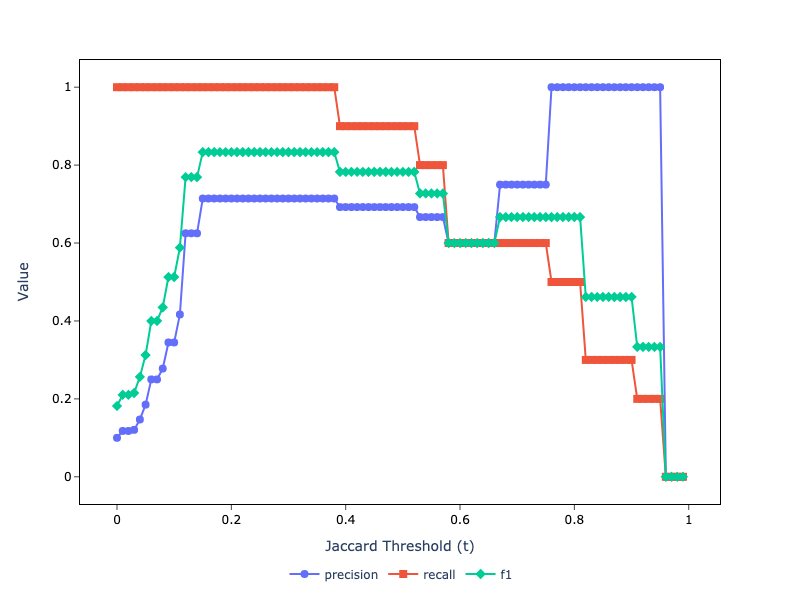
\includegraphics[width=\columnwidth]{mini-buy-fsm-main}
    \caption{Statistical metrics on `mini-buy' dataset
    \textcolor{green}{for results of F-S model}
    }
    \label{fig:mini-buy-fs}
\end{figure}

We can make some observations based on Figure~\ref{fig:mini-buy-fs}.
For values of $t \geq 0.78$, we end up with fewer (lower recall), but more
accurate matches (higher precision) than compared to lower values of $t$ because
the amount of false positives decreases and the amount of false negatives
increases.

For $0.6 \leq t \le 0.78$, precision decreases because the false
positive rate increases and recall increases because the false negative rate
decreases.
This is in line with expectations: the prefix becomes shorter causing a higher
percentage of attributes to be identical.
However, the prefix length is not short enough so that some of the matching
entity references in the ground truth that are more different from one another
will also be captured by \texttt{ppjoin}.

Compared to the previous interval, for values of $0.36 \leq t \le 0.6$, both
precision and recall increase compared to the previous interval.
As the prefix drops, more and more items from the ground truth are matched.
The number of false negatives decreases while the number of false positives
does not increase as fast as the number of true positives.

When $t$ is nearing zero there is an expected increase in recall due to fewer
and fewer overall negatives.
Precision, expectedly decreases due to an ever higher false positive rate.

We need to make a small note on near-identical items in the control data set,
such as \texttt{208114672} and \texttt{208114673}.
For lower values of \textit{t}, the algorithm produces two true positives and
two false positives.
By itself, the increase in false positives intuitively lowers precision.
However, lower values of \textit{t} also broaden the comparison space which
now contains entity references with short values for the name attribute,
like \texttt{205554724}.
By having new items to compare, we also increase the amount of true positives.
This dynamic ends up increasing precision as we lower values of \textit{t} so
long as we are not operating on the full input set.

Note that while we do describe the dynamic specifically for the \texttt{ppjoin}
algorithm, the dynamic of having an increased number of true positives offset
precision in an unexpected direction is not algorithm specific at all.
Regardless of the algorithm that we use, given some circumstances specific for
that algorithm, it should be possible to obtain the same effect we see here.
This observation is interesting because most entity resolution users look at the
F1 score thinking that it provides a good balance between precision and recall.
These users rarely analyse the components of the F1 score.
This situation can lead to unexpected outcomes.
For instance, there might be a substantial drop in F1 scores, which are
indicators of accuracy, when the input data for the entity resolution process is
changed.
The reason for this is that the precision or recall may be higher than expected
for the ideal configuration determined in the controlled scenario.

On the other hand, a balanced trade-off between precision and recall might not
be a requirement.
For instance, a core legal principle applicable in many jurisdictions across the
world states that is far more favourable to let 100 guilty people escape than to
put one innocent behind bars.
By that logic, we only care about precision.
Perfect recall while still retaining some precision might be useful during
research (e.g~finding papers on the same topic) or medical diagnosis (other
cases with the same symptoms).
In these cases, sifting through false positives might be preferable to missing
out on important information because of a false negative that is due to a
suboptimal input configuration.

Our control dataset (which is purposefully flawed) instructs us that the ideal
configuration values for our algorithm are:
\begin{itemize}
    \item $0.15 \leq t \leq 0.38$ for the best balanced outcome
    \item $t \leq 0.38$ for the most sensitive system
    \item $0.76 \leq t \leq 0.95$ for the highest precision
\end{itemize}

\subsubsection{Pairwise Metrics}

The ground truth and the result of the ER process are represented as partitions
over an input set of data.
Because we include the IDs in both DG1 and DG2, the input data set will
contain 20 items.
The ground truth contains 10 pairs of items.

Measuring the similarity of two partitions can be accomplished in more ways than
measuring the statistical success of a matching process.
Among these metrics, the pairwise comparison of two partitions is the best
approximation of the statistical metrics\cite{Men10}.
Figure~\ref{fig:mini-alg-pairwise} shows the computed pairwise metrics for
various values of \textit{t}.

\begin{figure}[!h]
    \centering
    \captionsetup{justification=centering}
    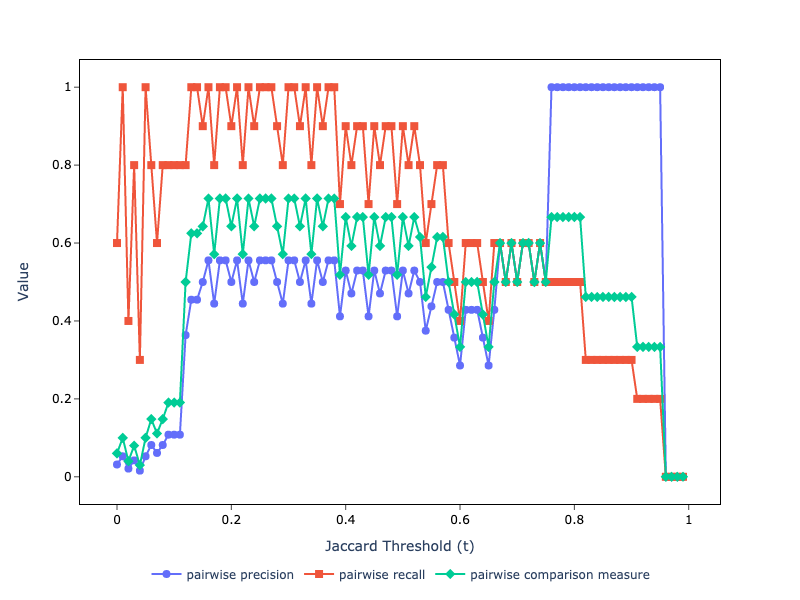
\includegraphics[width=\columnwidth]{mini-buy-algebraic-pairwise}
    \caption{Pairwise metrics on `mini-buy' dataset
    \textcolor{green}{for results of algebric model}\\
    \textcolor{green}{oare in legenda, la verde, nu ar tb sa fie pairwise F1?}
    }
    \label{fig:mini-alg-pairwise}
\end{figure}

We can see a plot similar to the one in Figure~\ref{fig:mini-buy-fs}.
The optimal range for high PF1 scores is the same to the case of statistical measures and the pairwise precision plot's shape
is almost identical (save for a smoother in the statistical model).

It is in terms of recall where we see a major difference from the statistical
model's plot.
More specifically, for $t \le 0.12$ pairwise recall drops significantly whereas
statistical recall stays at the maximum value.
The reason behind this variation lies in the difference between the two models of entity
resolution.
Whereas the standard recall formula only accounts for false negatives (of which
we can not have any using the generated data set), pairwise recall requires the
result data to be partitioned.
The partitioning operation removes any duplicates a partition class might
contain (such as duplicate matches returned by \texttt{ppjoin} for very low
values of \textit{t}).
Probabilistic recall seems to fail to adequately address situations where the
volume of data returned at the end of the entity resolution process vastly
exceeds the size of the ground truth, despite encompassing all true positives.
While in the context of a control dataset this may seem like an unlikely issue,
consider that for practical applications the size of the ground truth is often
several orders of magnitude smaller than the size of the input.

We note again that while the circumstances in which we show this behaviour are
specific to \texttt{ppjoin}, the phenomenon in itself is specific to the model
we employ when we evaluate the algorithm's performance.
Other algorithms may provide the conditions for this phenomenon using their own
input configurations.
To ensure a valid measurement system (one that is both accurate and precise), we
should collect pairwise metrics along with statistical metrics.

\subsubsection{Cluster Metrics}

Pairwise metrics are a form of measuring how well-formed the output of an entity
resolution task is.
The other widely spread family of metrics from this category that resembles
statistical metrics are the cluster metrics, which are displayed in
Figure~\ref{fig:mini-alg-cluster} for 'mini-buy' dataset.

\begin{figure}[!h]
    \centering
    \captionsetup{justification=centering}
    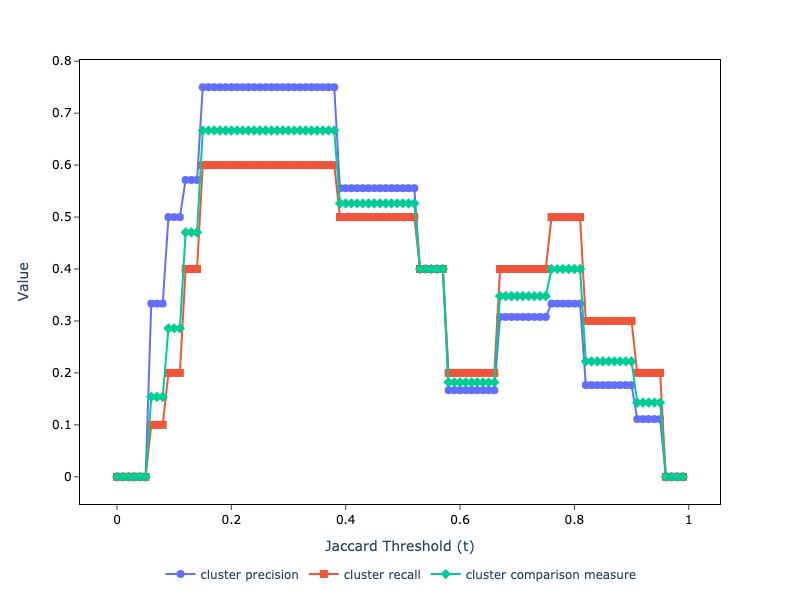
\includegraphics[width=\columnwidth]{mini-buy-algebraic-cluster}
    \caption{Cluster metrics on `mini-buy' dataset 
    \textcolor{green}{for results of algebric model}\\
    \textcolor{green}{oare in legenda, la verde, nu ar tb sa fie cluster F1? (stiu ca e sisnonim cu CCM, dar cand s-a dat formula a fost botezata CF1, iar in prima figura s-a facut referire tot la F1)}
    }
    \label{fig:mini-alg-cluster}
\end{figure}

It is refreshing to see that the optimal value of \textit{t} for a well-balanced
output should still be in the $\left[0.15,0.38\right]$ interval.
We also notice that cluster metrics point out the lack of recall when \textit{t}
nears zero even more than the pairwise metrics.
A more nuanced point is that recall decreases for $t \in \left[0.38,0.58\right]$
much more pronouncedly.

Clustering metrics also reveal interesting aspects about the other metrics we have
seen so far.
For example, we expect increased statistical and pairwise precision to
correspond to increased cluster precision.
This is only somewhat true.
As \textit{t} decreases, we see statistical and pairwise precision increasing
along with cluster precision.
What is interesting is just how much cluster precision increases.
As \textit{t} decreases, more and larger clusters are returned by the entity
resolution task.
For a series of values of \textit{t} the number of returned clusters does not
change much, while the shape of the partition returned by the entity resolution
task becomes more and more similar to the shape of the ground truth.
As the entity resolution task starts returning larger and larger clusters, the
cluster precision drops significantly even though the number of clusters
returned by the entity resolution task drops as well.

A similar effect can be observed for cluster recall as we increase the value of
\textit{t}.
When statistical precision increases, there is a good chance that the number of
clusters in the entity resolution result which are in agreement with the ground
truth would also increase.
Because there are fewer matches as statistical precision increases, we have a
partition that contains many singletons.
This causes cluster precision to decrease (because it relates to the number of
clusters returned by the entity resolution task) and cluster recall to increase
(because it relates to the number of clusters in the ground truth which remains
constant).

These phenomena do not depend on the entity resolution algorithm, but are
characteristics of cluster precision and cluster recall.
Higher statistical recall will always mean fewer and larger clusters some of
which will overlap with clusters in the ground truth.
Higher statistical precision will always mean more singleton clusters returned
by the entity resolution task which, in turn, will increase cluster recall.

Remembering that we might not care about balanced output, we can consider
cluster precision and cluster recall as metrics that balance out the bias built
into statistical precision and recall.
Furthermore, cluster precision and recall can also be used together with
pairwise metrics to confirm any blind spots in the statistical metrics.

In our own practical example, we will use these findings to keep an eye on
$t\in\left[0.76,0.81\right]$ as an interesting input configuration when we are
biased towards better precision.

\subsubsection{Clustering Indexes}

Even though pairwise and cluster metrics complement the statistical metrics,
sometimes all we want is a clear picture of the optimal input configurations for
the algorithm.
The easiest way to glean this information is by using one of the clustering
indexes depicted in Figure~\ref{fig:mini-alg}.

\begin{figure}[!h]
    \centering
    \captionsetup{justification=centering}
    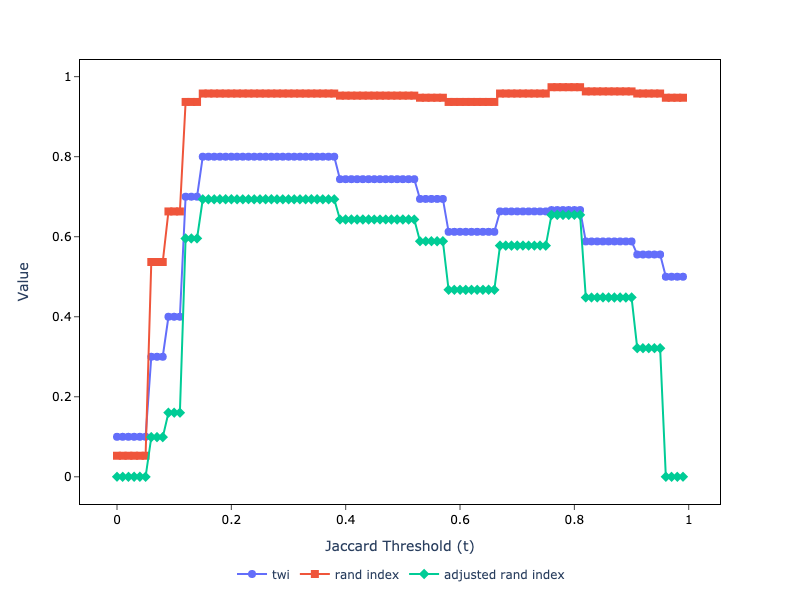
\includegraphics[width=\columnwidth]{mini-buy-algebraic-main}
    \caption{Clustering indexes on `mini-buy' dataset}
    \label{fig:mini-alg}
\end{figure}

We observe that the plot of the Adjusted Rand Index indicates both the desirable
and the undesirable values of \textit{t}.
Notice that it ranks $t\in\left[0.76,0.81\right]$ almost as highly as
$t\in\left[0.15,0.38\right]$.
By following its plot, we should stay clear of values of \textit{t} from other
intervals --- especially those at the extremities of the definition interval.

By comparison with the ARI, the Rand Index itself is not very informative.
It signals that recall is not perfect for values of \textit{t} nearing zero and
does give the highest score for $t\in\left[0.76,0.81\right]$.
However, it also gives high scores for values of \textit{t} where all the other
metrics do not.

The Talburt-Wang index's plot is a fairly good indicator, taking all our former
observations into account.
The only aspect where it is lagging is for $t\in\left[0.76,0.81\right]$.
Here it fails to clarify the favorable circumstances due to high statistical
precision and high cluster recall.

The Adjusted Rand Index or, if operational performance is key, the Talburt-Wang
Index provide enough meaningful information to find ballpark figures for ideal
configuration settings for an entity resolution task.

\subsection{Outcomes from Benchmark Datasets}\label{subsec:experiment-benchmark}

So far we have seen evidence on the generated miniature dataset that each
theoretical model provides a lens through which we can interpret various aspects
of an entity resolution task's qualitative performance.
Some invariants with respect to the entity resolution task have been discovered.
Nothing related to the task that is being evaluated determines these phenomena.
However, we don't know if any of them are invariant with respect to the data
being used.

We want to understand if there are conditions or phenomena that could help us
extract universally good input configurations for an entity resolution algorithm
by using a small dataset.
There already seem to exist some interesting relationships between metrics
including a blind spot in how statistical recall is computed regardless of the
used entity resolution algorithm.
Now we have to see if any of them persist if we change the data used for
performing entity resolution.

In order to do this we shall use benchmark datasets.
The first of these is the `Abt-Buy' data set~\cite{vldb2010} and the plots for
our experiment are available in Figures~\ref{fig:abt-buy-fsm-main},
~\ref{fig:abt-buy-algebraic-pairwise},~\ref{fig:abt-buy-algebraic-cluster}
and~\ref{fig:abt-buy-algebraic-main}.

\begin{figure*}[ht]
    \begin{minipage}{0.24\textwidth}
        \centering
        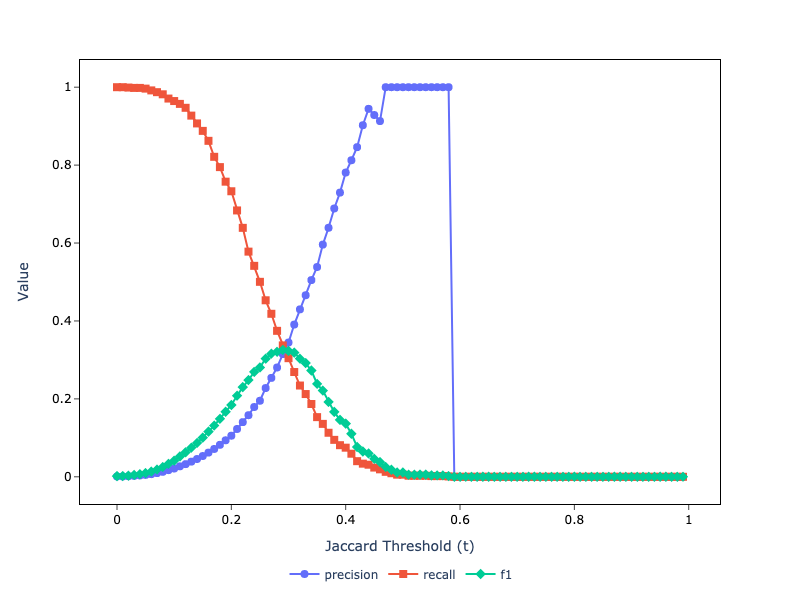
\includegraphics[width=\textwidth]{abt-buy-fsm-main}
        \caption{Abt-Buy statistical metrics.}
        \label{fig:abt-buy-fsm-main}
    \end{minipage}
    \begin{minipage}{0.24\textwidth}
        \centering
        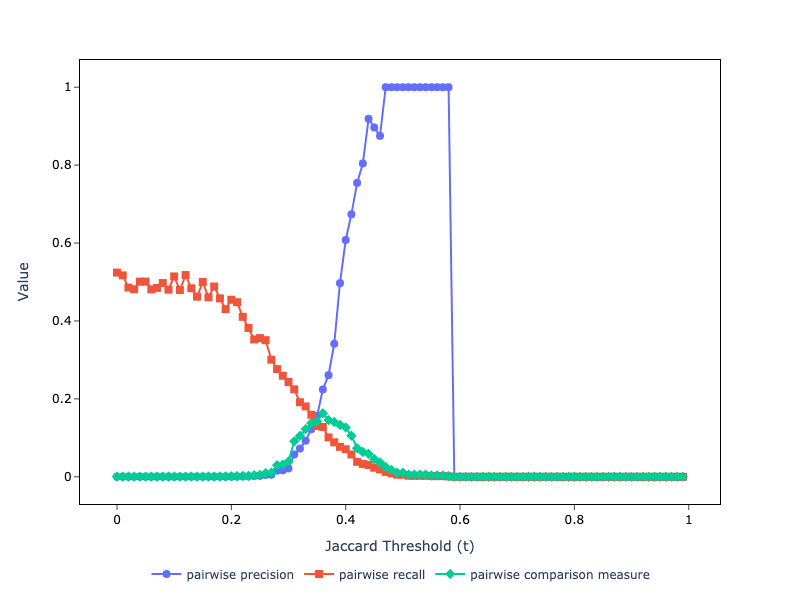
\includegraphics[width=\textwidth]{abt-buy-algebraic-pairwise}
        \caption{Abt-Buy pairwise metrics.}
        \label{fig:abt-buy-algebraic-pairwise}
    \end{minipage}
    \begin{minipage}{0.24\textwidth}
        \centering
        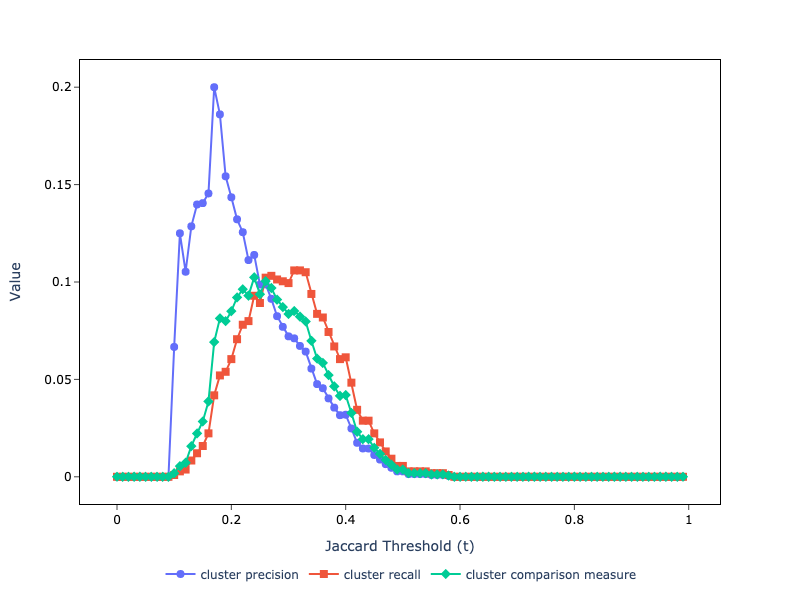
\includegraphics[width=\textwidth]{abt-buy-algebraic-cluster}
        \caption{Abt-Buy cluster metrics.}
        \label{fig:abt-buy-algebraic-cluster}
    \end{minipage}
    \begin{minipage}{0.24\textwidth}
        \centering
        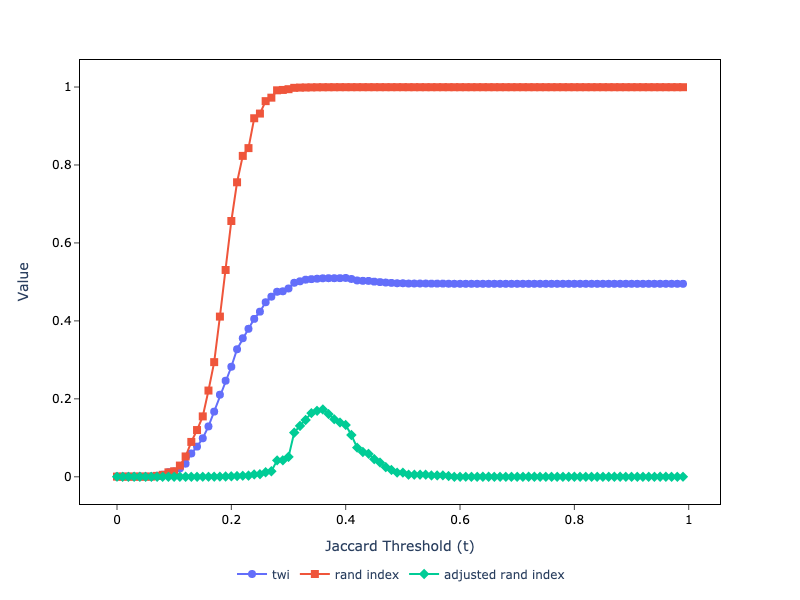
\includegraphics[width=\textwidth]{abt-buy-algebraic-main}
        \caption{Abt-Buy clustering indexes.}
        \label{fig:abt-buy-algebraic-main}
    \end{minipage}
\end{figure*}\label{abt-buy}

We can see that the statistical model still has a pronounced bias towards higher
recall values.
The other invariant that also seems to hold for this dataset as well is the
balancing/confirmation action of the cluster metrics with respect to the
statistical/pairwise metrics.
Another nice confirmation is that the pairwise recall is never perfect.
Lastly, the clustering indexes are good approximates of the ballpark where
we could find  interesting input configurations.
All interesting values of \textit{t} 
\textcolor{green}{I would indicate the value or the value's range for this optimal $t$} 
are in the ballpark indicated by these
indexes.

On the other hand, we can clearly see that input configurations 
\textcolor{green}{la ce anume te referi prin aceste "input configs"? Ai mai amintit si mai devreme, dar nicaieri nu e specifica clar la ce anume se refera; e vorba doar de pagrul $t$ sau si de algoritm de ER si alti params?}  
such as those
that take advantage of a high precision to high cluster recall correlation are
dataset specific.

We move on to the `Amazon-Google Products' data set~\cite{vldb2010} and observe
the results in Figures~\ref{fig:amazon-googleproducts-fsm-main},
\ref{fig:amazon-googleproducts-algebraic-pairwise},
\ref{fig:amazon-googleproducts-algebraic-cluster} and
\ref{fig:amazon-googleproducts-algebraic-main}.

\begin{figure*}[h]
    \begin{minipage}{0.24\textwidth}
        \centering
        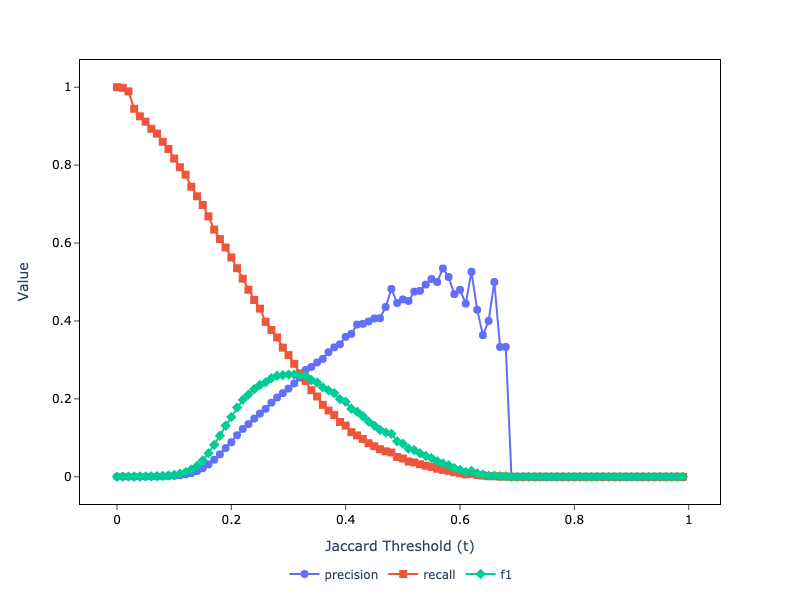
\includegraphics[width=\textwidth]{amazon-googleproducts-fsm-main}
        \caption{Amazon-Google statistical metrics.}
        \label{fig:amazon-googleproducts-fsm-main}
    \end{minipage}
    \begin{minipage}{0.24\textwidth}
        \centering
        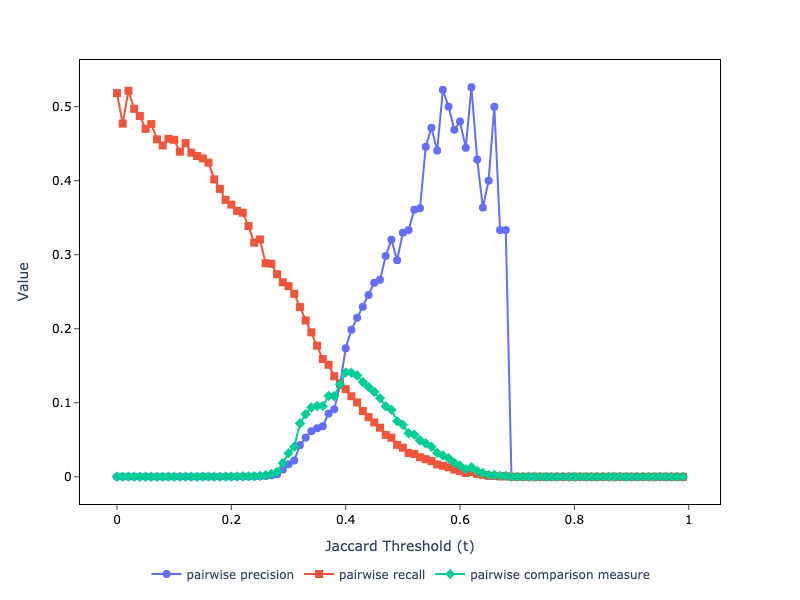
\includegraphics[width=\textwidth]{amazon-googleproducts-algebraic-pairwise}
        \caption{Amazon-Google pairwise metrics.}
        \label{fig:amazon-googleproducts-algebraic-pairwise}
    \end{minipage}
    \begin{minipage}{0.24\textwidth}
        \centering
        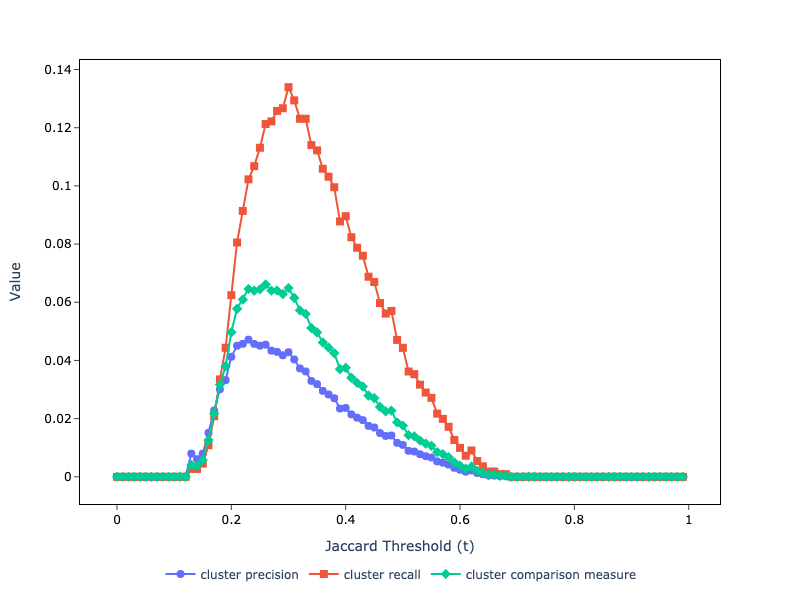
\includegraphics[width=\textwidth]{amazon-googleproducts-algebraic-cluster}
        \caption{Amazon-Google cluster metrics.}
        \label{fig:amazon-googleproducts-algebraic-cluster}
    \end{minipage}
    \begin{minipage}{0.24\textwidth}
        \centering
        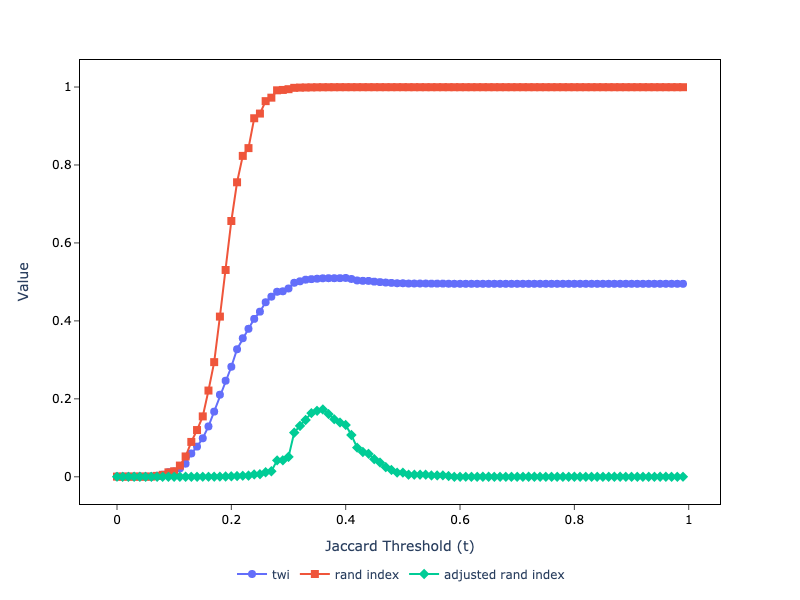
\includegraphics[width=\textwidth]{abt-buy-algebraic-main}
        \caption{Amazon-Google clustering indexes.}
        \label{fig:amazon-googleproducts-algebraic-main}
    \end{minipage}
\end{figure*}\label{amazon-google}

The plotted data shows that the statistical model is biased toward high recall
in this data set, also.
It also shows that pairwise metrics show lower score for recall while
maintaining the shape of the plot for statistical metrics.
Albeit less clearly, we still see that cluster precision and cluster recall can
still act as a balancing weight or confirmation for the statistical metrics or
pairwise metrics, respectively.

On the other hand, we start seeing that the clustering indexes are no longer
individually indicating a ballpark correctly.
The Talburt-Wang index seems to indicate the same optimal input configuration as
the cluster metrics, whereas the Adjusted Rand Index seems to provide a ballpark
of optimal input configurations that would also maximize scores obtained for
pairwise metrics and statistical metrics.
Even though one can assume that this is because of how the two indexes are
defined (TWI counts agreements on whole clusters while ARI counts agreeing
pairs), confirming this assumption experimentally requires further work.
Regardless, we can safely conclude that whether clustering indexes reveal
ballparks for optimal input configurations is dataset dependent.
\textcolor{green}{mie nu mi-e clar ce ai vrut sa spui :(}

Finally, we look at the `DBLP-ACM' benchmark dataset~\cite{vldb2010}.
The plots we obtained after running the experiment on this dataset are available
in Figures~\ref{fig:dblp2-acm-fsm-main},
\ref{fig:dblp2-acm-algebraic-pairwise},
\ref{fig:dblp2-acm-algebraic-cluster} and
\ref{fig:dblp2-acm-algebraic-main}.

\begin{figure*}[h]
    \begin{minipage}{0.24\textwidth}
        \centering
        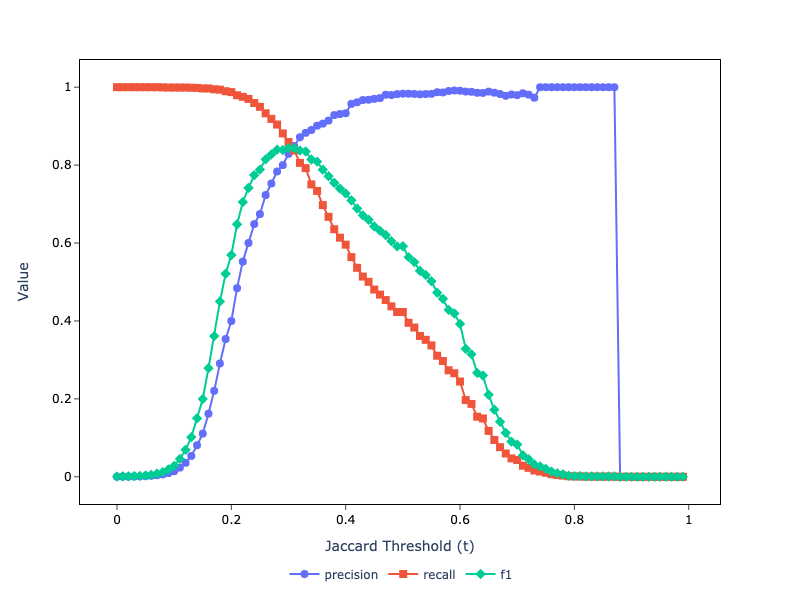
\includegraphics[width=\textwidth]{dblp2-acm-fsm-main}
        \caption{DBLP-ACM statistical metrics.}
        \label{fig:dblp2-acm-fsm-main}
    \end{minipage}
    \begin{minipage}{0.24\textwidth}
        \centering
        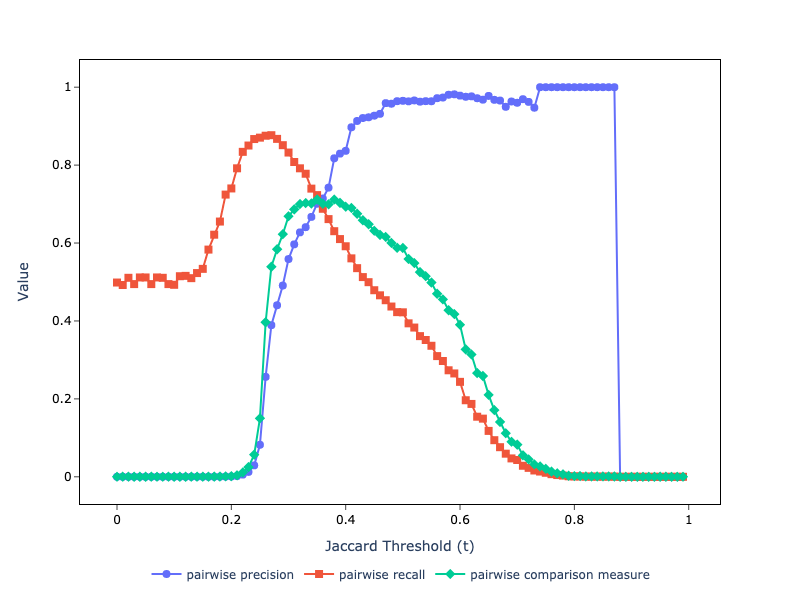
\includegraphics[width=\textwidth]{dblp2-acm-algebraic-pairwise}
        \caption{DBLP-ACM pairwise metrics.}
        \label{fig:dblp2-acm-algebraic-pairwise}
    \end{minipage}
    \begin{minipage}{0.24\textwidth}
        \centering
        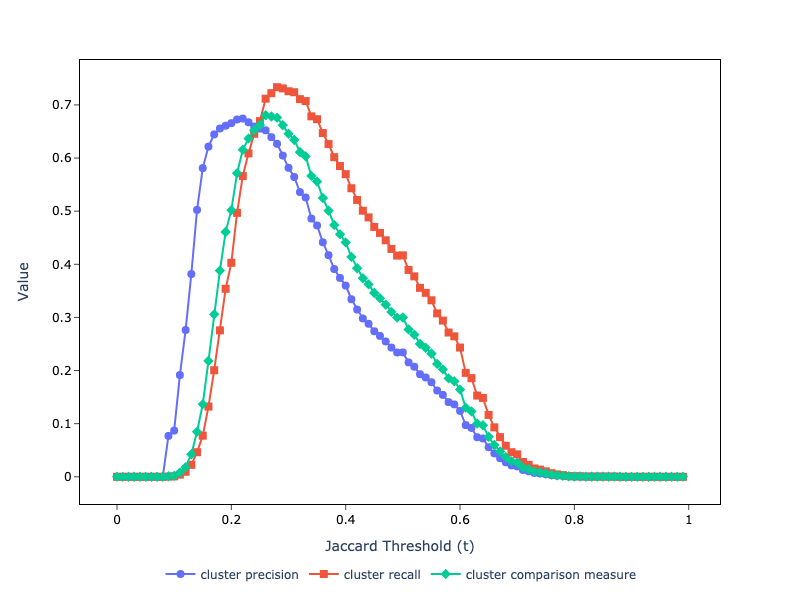
\includegraphics[width=\textwidth]{dblp2-acm-algebraic-cluster}
        \caption{DBLP-ACM cluster metrics.}
        \label{fig:dblp2-acm-algebraic-cluster}
    \end{minipage}
    \begin{minipage}{0.24\textwidth}
        \centering
        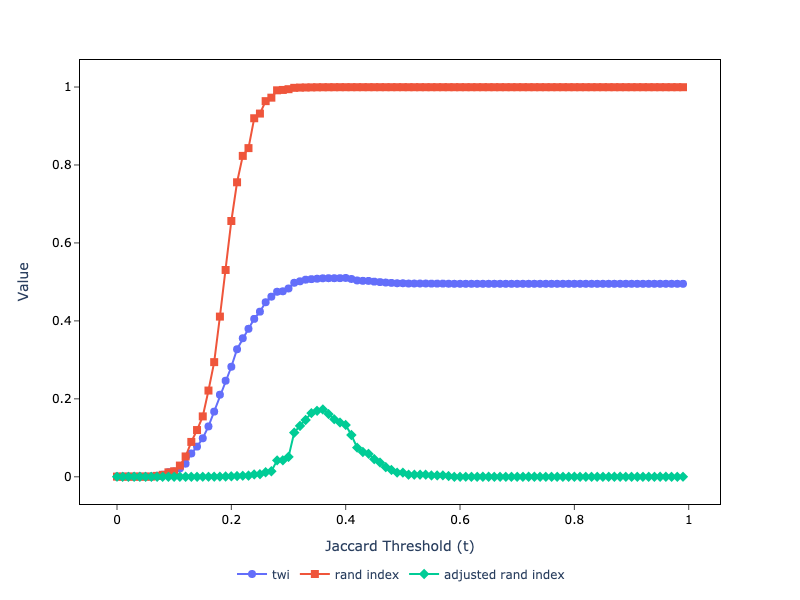
\includegraphics[width=\textwidth]{abt-buy-algebraic-main}
        \caption{DBLP-ACM clustering indexes.}
        \label{fig:dblp2-acm-algebraic-main}
    \end{minipage}
\end{figure*}\label{dblp2-acm}

Looking at the plots for this last dataset we again see confirmation that recall
in the statistical model is much higher than advertised by any of the other
metrics.
The other condition that is invariant with respect to the algorithm and the
data sets is that cluster precision and cluster recall act as good balancing or
confirmation metrics for the statistical and pairwise metrics, respectively.
\textcolor{green}{mie nu mi-e clar ce ai vrut sa spui :(}

We also see that the conjecture concerning the TWI as a good approximation for
input configurations that yield high clustering scores holds for this data set,
too. 
The same can be said about the ARI for approximating high scores with regard to
matching.
These observations hold for all four datasets we have experimented on.


\textcolor{green}{As incerca sa le enunt din nou acest concluzii, iar dupa ce sunt formulate le-as transforma in ipoteze, descriindu-le la inceputul sectiunii cu experimentele; astfel, ele vor reprezenta motivatia: avem 3-4 hipoteze si ne propunem sa le validam prin experimentele efectuate . Eu am retinut asa: \\
1. hypothesis about precision - TBA \\
2. recall in the statistical model is much higher than advertised by any of the other metrics.\\
3. cluster precision and cluster recall act as good balancing or
confirmation metrics for the statistical and pairwise metrics, respectively.\\
4. TWI is a good approximation for input configurations that yield high clustering scores.\\
5. ARI - ???\\
6. ???
}



    \section[conclusion]{Conclusions}\label{sec:conclusions}

    \textcolor{green}{tb adaugata o fraza despre context (ER) si scipul mare al studiului. Abia apoi vin evidentiate cele 2 mari concluzii/zontributii: maparea unui model in altul si analiza dpdv al metricilor}

    In this paper we have provided an overview of how theoretical models for
    entity resolution influence the data structures that are at play when we are
    working with entity resolution systems in practice.
    The data structures involved using the Fellegi-Sunter model for entity
    resolution revolve around pairs of entity references, whereas those that
    are specific to the algebraic model are centered around sets and partitions
    over sets.
    One interesting finding is that a transition from the Fellegi-Sunter model
    to the algebraic model is possible using the Union-Find data structure and
    a simplified version of Kruskal's algorithm.

    Having this knowledge we ran an experiment using the \texttt{ppjoin}
    algorithm on a generated data set.
    By looking at the results we saw how theoretical models provide different
    perspectives on the same algorithm.
    Having this outlook on things, we were able to glean insights that have
    nothing to do with the algorithm but with the perspectives themselves.

    To see whether the perspectives change if the underlying data changes, we
    ran the experiment on three different benchmark datasets.
    A first conjecture that arises after doing so states that the Fellegi-Sunter
    model for entity resolution provides a perspective over the quality of the
    entity resolution results which is overly optimistic in evaluating recall.
    This leads to higher F1 scores and possibly to wrong conclusions when
    comparing entity resolution solutions using the F1 score.

    The second conjecture is that we can safely use the Talburt-Wang Index to
    find input configurations of the entity resolution task in which it performs
    clustering well.
    The Adjusted Rand Index can be used in the same way to find input conditions
    where the entity resolution task performs matching well.

    We will not draw any conclusion with regard to extrapolating observations on
    smaller sets to larger sets of data or to the overall performance of the
    algorithm even though the data suggests that at least the ballpark stays the
    same.
    In order to make such claims, we need to design and run experiments using
    other entity resolution algorithms.

    \section[future]{Future Work}\label{sec:future}

    In terms of theory, we would like to consider other models for entity
    resolution.
    Firstly, there is existing models such as the one proposed by the Stanford
    Entity Resolution Framework\cite{Ben2009Swoosh} or the graph theoretical
    model of entity resolution which is widely used in entity alignment tasks.
    Then there are theoretical models that we can imagine in the realms of
    recommender systems or a retrieval augmented generative AI.

    The other route to take is to run experiments using more and more algorithms
    to find out whether the conjectures outlined in this paper are worth proving.
    Given the costs of fine-tuning an entity resolution system, a good step
    forward seems to be finding some invariants that would allow us to test
    the system with smaller datasets.

    Lastly, this paper was about finding invariants in the realm of qualitative
    measurements of entity resolution tasks.
    Implementing a system that shows the qualitative and quantitative metrics
    of any entity resolution task would make adopting and tuning entity
    resolution systems less costly and more transparent.


    \textcolor{green}{things that are confused:\\
    1. model vs. algorithm vs. task related to ER\\
    2. scopul art: sa evidentiem mapparea FS vs model algebric sau sa analizam critic metricile (pt ca doar astfel se poate face o alegere eficienta a modelului de ER folosit, desi tb tinut cont ca suntem intr-un mediu oarecum controlat; unde avem niste dataset-uri limitate, nu de tip openworld pt care nu se calculeaza efectiv metricile, ci se estimeaza cumva - a se vedea problema despre bridging
    the reality-ideality gap in entity resolution, where high performance on benchmark datasets often does not
    translate into the real world \href{https://arxiv.org/pdf/2205.05889.pdf}{link}) sau ambele? :D\\
    3. in fc de scopul de la pct 2 tb adaugat in introducere info despre contributie, precum si in Rel Work\\
    4. def pt "perspectiva" (de sine statatoare sau relativ la un model sau la un algo de ER); \\
    5. def pt "input config" \\
    6. de verificat daca folosirea notiunii de "invariant" se poate demonstra si teoretic, nu doar empiric\\
    7. relatia cu RelWork (ce e comun, ce e diferit cu alte lucrari care abordeaza maparea unui model in altul, respectiv evaluarea prin metrici); de vazut lucrari precum:\\
    https://arxiv.org/pdf/2107.10590.pdf \\
    https://arxiv.org/pdf/1509.04238.pdf\\
    http://honors.cs.umd.edu/reports/hitesh.pdf\\
    https://arxiv.org/pdf/2210.01230.pdf\\
    8. tb spus de ce nu s-au inclus si alte metrici (de ex GMD)\\
    9. tb spus ceva despre class imbalance (ce influenta are asupra metricilor faptul ca sunt doar cateva elemente aliniate/duplicate si multe elemente nealiniate)\\
    10.
    }
    
    \bibliographystyle{ieeetr}
    \bibliography{er-general,er-related-work,er-additional-references,er-software}
\end{document}
